\documentclass{article}
\usepackage[english]{babel}
\usepackage[utf8]{inputenc}
\usepackage[table]{xcolor}
\usepackage{graphicx}
\usepackage{float}
\usepackage{longtable}
\usepackage{booktabs}
\usepackage{caption}

\usepackage{hyperref}
\hypersetup{
	colorlinks,
	citecolor=black,
	filecolor=black,
	linkcolor=black,
	urlcolor=black
}


\begin{document}


\begin{titlepage}
      \centering
      \begin{figure}
            \begin{center}
                  
\includegraphics[width=0.6\textwidth]{images/logo_polimi.png}
            \end{center}
      \end{figure}
      \vfill
      {\scshape\LARGE Software Engineering 2 Project\\Academic Year 2021 - 2022 \par}
      \vspace{0.8cm}
      {\scshape\LARGE DREAM}
      \vfill
      \newcommand{\HRule}{\rule{\linewidth}{0.3mm}}
      \centering
      \HRule \\[0.4cm]
      \huge  Requirements Analysis\\ and Specifications Document\\% Title of your document
      \HRule \\
      \vspace{1cm}
      {\Large Valeria \textsc{Detomas} \quad Sofia \textsc{Martellozzo} \par}
      \vfill
      {\large Professor\par
          Elisabetta \textsc{Di Nitto}}
      \vfill
      {\large \textbf{Version 1}\\ \today \par}
\end{titlepage}


\newpage
\renewcommand\contentsname{Contents}
\tableofcontents

\newpage

%-----------------------------------------------------------%
\section{Introduction}
\subsection{Purpose}
The purpose of this document is to thoroughly describe 
Data-dRiven PrEdictive FArMing in Telengana(DREAM).
It presents functional and non functional requirements of the system and its components.
Moreover it provides use cases and scenarios for the users involved.
\\This document is meant as a contractual basis for the customer and the developer.

\subsubsection{Goals}\label{section:1.1.1}
  \begin{table}[h]
        \rowcolors{1}{gray!25}{white}  
        \centering
  \begin{tabular}{|p{2cm}|p{9cm}|}
    \hline
    G1 & allow policy makers to retrieve information from farmers and to evaluate their performance\\
    \hline
    G2 & allow farmers to communicate with each other\\
    \hline
    G3 & allow farmers to insert data and advices on his production\\
    \hline
    G4 & allow farmers to send request of help to Policy Makers\\
    \hline
    G5 & allow farmers to retrieve information relevant for their activity\\
    \hline
    G6 & Policy Makers and farmers should be able to consult the map of the zone ( and the informations stored in it ) with different levels of visibility\\
    \hline
    G6A & Policy Makers and farmers should be able to see the position of the farms on the map\\
    \hline
    G6B & Policy Makers should be able to see both the information about the production and the evaluation of each farm\\
    \hline
    G6C & farmers should be able to see only the type of production of a farmer by the map\\
    \hline
  \end{tabular}
  \caption{Definition of goals}
\end{table}

\subsection{Scope}

The aim of the system is to acquire and combine data and information of farmers in Telengana. 
The system will provide support both to Telengana’s policy makers and to farmers 
thanks to new innovative technologies.\\
Through the system, policy makers are able 
to get a complete picture of the agriculture status in the whole state. In order 
to obtain this, Dream provides information that make policy makers able to give 
incentives to those farmers who are performing well. Moreover it allows them to 
keep track of those farmers who need help. \\
The farmers have access to a forum where they are able to communicate with other 
farmers. The aim of the forum is to share useful suggestions and to let farmers 
who struggle with something ask for help. \\
Therefore on the one side policy makers can have an entire perspective of the farms’ 
situation in the entire state and on the other side farmers can take advantage of the 
application and discuss with their colleagues.
\par 
Hence the application is used by the policy makers as a way to monitor farmers. 
Through the system they are able to search a farm and have access to its general information. 
Once a month they salso end each farmer an evaluation message where they specify if the farmer activity was
performed good or bad.\\
On the contrary farmers can ask for help or write advices. They are free to write messages and communicate with other farmers through a forum 
that is created especially for them.




\subsubsection{World Phenomena}
\begin{itemize}
    \item Farmer starts growing some type of crop
    \item Weather conditions influence production
    \item Telengana’s state collects data concerning meteorological forecasts
    \item Farmer uses water irrigation system
    \item Farmer is struggling with his harvest  
    
\end{itemize}

\subsubsection{Shared Phenomena}

\begin{itemize}
    \item Farmer access Dream
    \item Farmer sends a message in the forum
    \item The amount of water used by the farmer is registered on the application
    \item Farmer inserts data about his production in the system
    \item Farmer sends a help request to the policy maker
    \item A user visualizes the map that identifies the farms
    \item Policy maker evaluates farmers' performances
    \item A user checks notifications
    
\end{itemize}

\subsection{Glossary}
\subsubsection{Definitions}
\begin{itemize}
        \item \textbf{DBMS} is a software that works as an interface between the end user and the database. It manages the data, the database engine and the database schema.
        \item \textbf{HTTPS} is a protocol where encrypted HTTP data is transferred over a secure connection. It also guarantees the privacy and integrity of data.
        \item \textbf{API} is a programming code that helps communicate two different computer programmes.
\end{itemize}
\subsubsection{Acronyms}
\begin{itemize}
        \item \textbf{API}: Application Programming Interface
        \item \textbf{HTTPS}: Hypertext Transfer Protocol Secure
        \item \textbf{DBMS}: Data Base Management System
        \item \textbf{UML}: Unified Modelling Language
\end{itemize}
\subsubsection{Abbreviations}
\begin{itemize}
        \item \textbf{Gn} goal number n
        \item \textbf{Rn} requirement number n
        \item \textbf{DAn} domain assumption number n
        \item \textbf{UCn} use case number n
        \item \textbf{Sn} scenario number n
\end{itemize}

\subsection{Document Structure}
\begin{enumerate}
    \item \textbf{Introduction}\\
            This section offers an introduction and a brief overview of the system that is presented in the document. 
            It highlights the purpose of the system and the goals that are meant to be achieved with it. 
            At the end there is also a glossary that contains a list of definitions, acronyms and abbreviations.
            
    \item \textbf{Overall Description}\\
            This section starts with a product perspective that contains a description of the system's domain through a class diagram. 
            It includes also state diagrams which are used to give more details about the behavior of some objects in the model.
            The section contains also a clear description of the features offered by the system, 
            it identifies the actors involved and it describes their characteristics.
            At the end there are domain assumptions and general constraints.
            
    
    \item \textbf{Specif Requirements}\\
            This section enters into the details on how the system interacts with the external world. It describes 
            the interfaces that are required and offered through several visual mockups. 
            Moreover the section provides functional and nonfunctional requirements. Functional
            requirements are additionally described by use cases, sequence diagrams and scenarios.
            At the end the section focuses on nonfunctional requirements and various limitations that the system might face.

    \item \textbf{Formal Analysis using Alloy}\\
            This section provides the model described through Alloy language.
            
    \item \textbf{Effor Spent}\\
            This section has a record of the hours spent to complete this document.

\end{enumerate}




%-----------------------------------------------------------%
\newpage
\section{Overall Description}
\subsection{Product Perspective}
\subsubsection{Class Diagram}
The class diagram represented in Figure~\ref{fig:uml} represents the domain of the system. \\
The main elements in the class diagram are:
\begin{itemize}
    \item \textbf{User}: identifies two types of users who can access the application.\\
    \textsl{Farmer} and \textsl{Policy Maker} are the two categories of users that are present in the system. \\
    The distinction has to be applied in order to have different permissions.\\
    Both have a password used for the autentication and an email, in the case of a farmer, or an alphanumeric code owned by a policy maker.
    \item \textbf{Farm}: stores all the information related to a Farm.\\ 
    It can be owned only by a farmer, and is located in a specific position visible by the map. \\
    It contains also the data about the production inserted by the farmer himself, that could be not present yet.
    (if a farmer has not started yet or has not inserted these information).\\
    Each farm is provided of sensors of two kind: one that collect data about the amount of water used by the farmer in his farm and humidity every day.\\
    \item \textbf{Notification}: this class represents content sent between users (in order to communicate something) or something submitted in the sistem that is stored in the database.\\
        \begin{enumerate}
            \item \textsl{Help}: it stores the single farmer that writes it, 
            the type of production he selects and a body where hthe farmer explains in details the problem.\\
            When this notification is sent (to the policy makers) the system registers in it the actual date and time.
            \item \textsl{Advice}: the structure of it is the same as the Help class but it is not sent to anyone,
             it is immediatly stored in the database.
            \item \textsl{Evaluation}: this class represents the evaluation on exacly one farm by a single policy maker.\\ Each policy maker can evaluate one or more 
            farms more than once since this event happens once a month.\\ Despite it, an evaluation is related only to one farm and the result can be positive (1) or negative (0).\\ The evaluation is sent by the policy maker to the farm owner.
            \item \textsl{Solution}: this class is like the Help one, in fact is the reply of a policy maker to a help request (by Help notification) from a farmer with in the body the solution found by the sender.
        \end{enumerate}
    \item \textbf{Evaluation}:
    \item \textbf{Map}: this object contains a list of all the farms located in Telegana and registered in the application.\\It stores all the information about the farms due to provides them to the users (in different ways).
    \item \textbf{Weather Info}: this class is a rapresentation of the meteorological information of the country, provided by an external application.\\These information are specific for each position in which is located a farm.
    \item \textbf{Production}:
    \item \textbf{Forum}:
    \item \textbf{SensorsData}
\end{itemize}
\begin{figure}[H]
    \begin{center}
    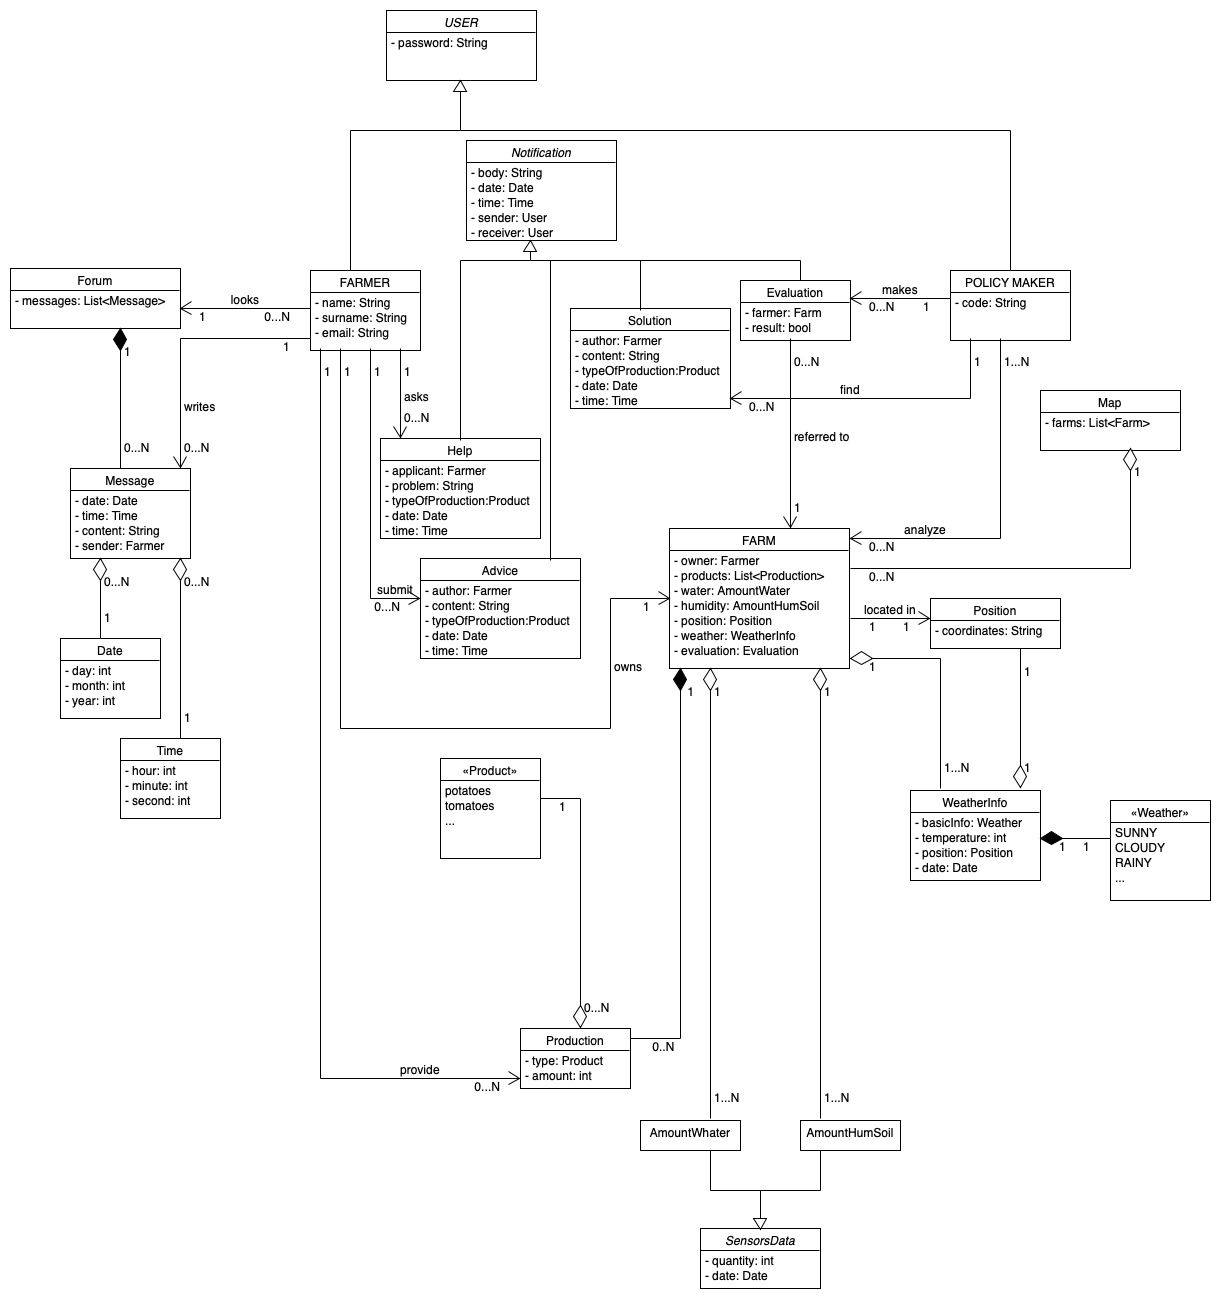
\includegraphics[width=1\textwidth]{images/UMLSW2_2.png}
    \caption{UML diagram.}
    \label{fig:uml}
    \end{center}
\end{figure}
\newpage
\subsubsection{State Diagrams}
The following state diagrams describe the behavior of the main objects of the system's domain previously described(Figure~\ref{fig:uml}). 
They consider all the potentional states that the element examined can have 
while a certain event takes place.

\begin{enumerate}
    \item \textbf{Update of the Farmer Page}
        The state diagram represented in figure~\ref{fig:state1} represents 
        the events that might occur whenever the farmer page is updated.
        The three main circumstances when the page is updated are:
        \begin {itemize}
        \item Farmer inserts new production data
        \item Every day the weather forecast is updated with the new data available on it
        \item Data collected from sensors are always up to date
        \end{itemize}
        The page is so update after one of this events occurs.

    \begin{figure}[H]
        \begin{center}
        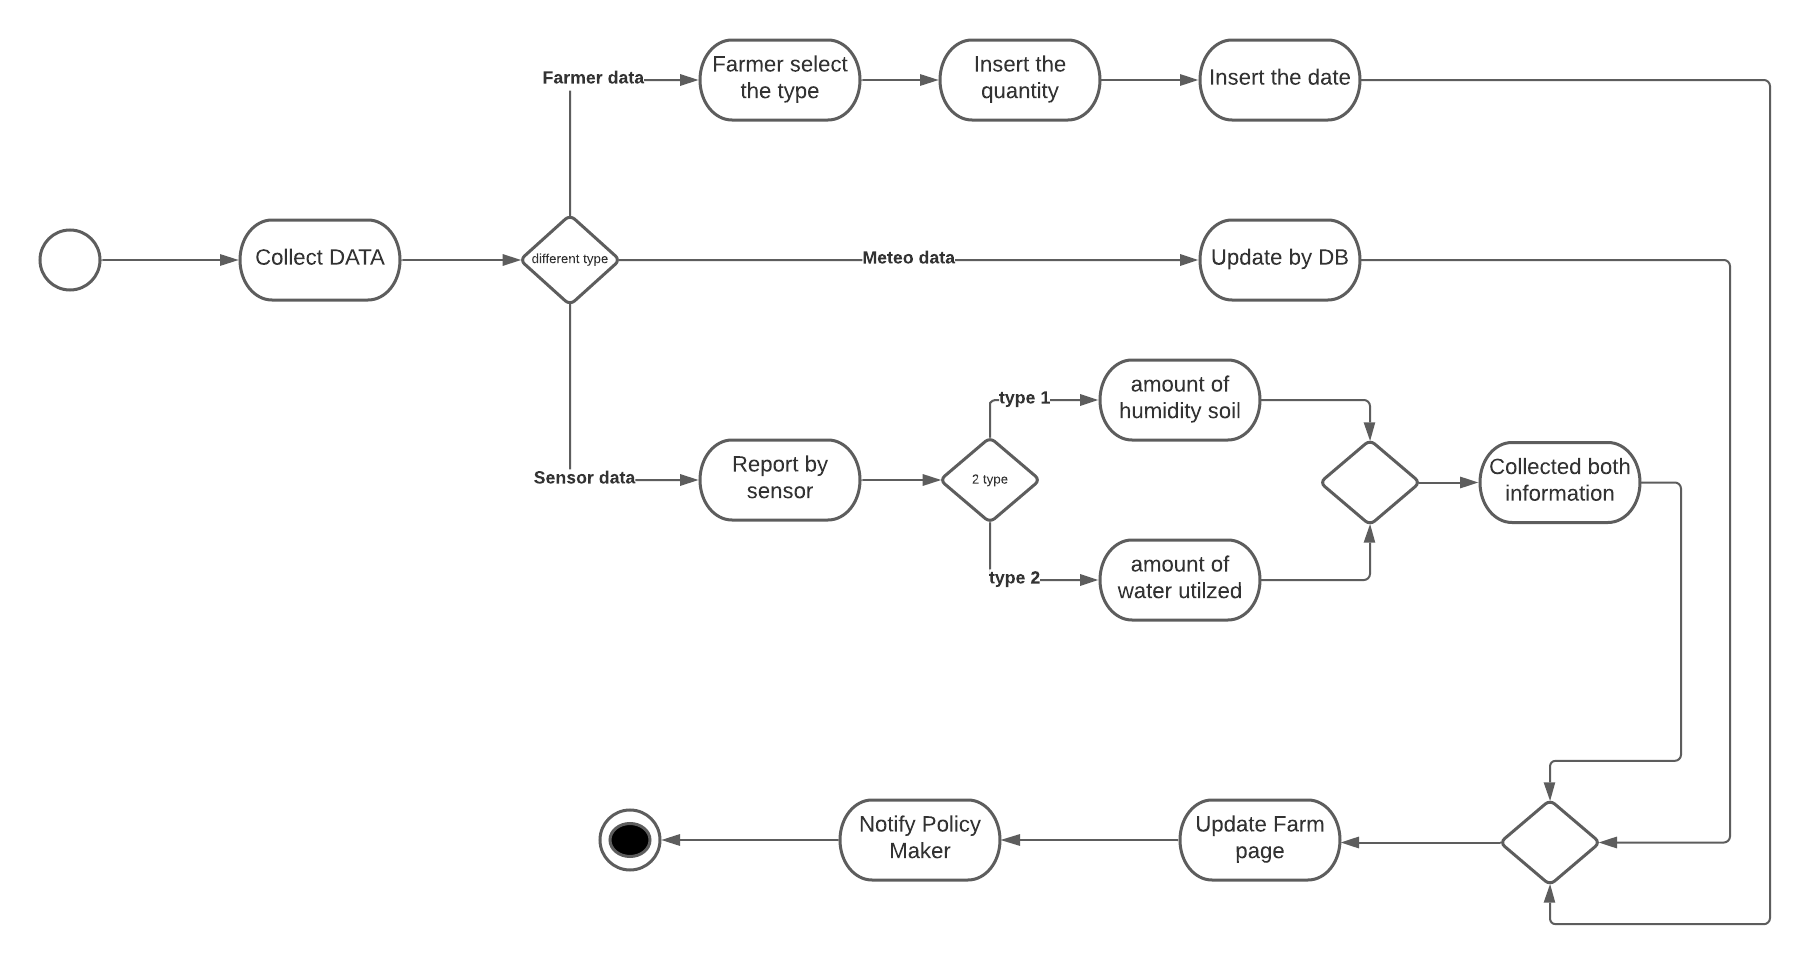
\includegraphics[width=1\textwidth]{images/State chart 1.png}
        \caption{Update Farmer page.}
        \label{fig:state1}
        \end{center}
    \end{figure}

    \item \textbf{Analysis of different farmers}
    The state diagram in figure \ref{fig:state2} represents the analysis that is performed 
    by the policy makers once a month.
    As a matter of fact the policy maker starts the analysis after selecting the farm, he visualizes then the farmer's farm page and analyzes the information 
    that is present in it. After the anlaysis the map is updated and the system sends a notification, that is then different if the 
    farmer’s performance is either good or bad.

    \begin{figure}[H]
        \begin{center}
        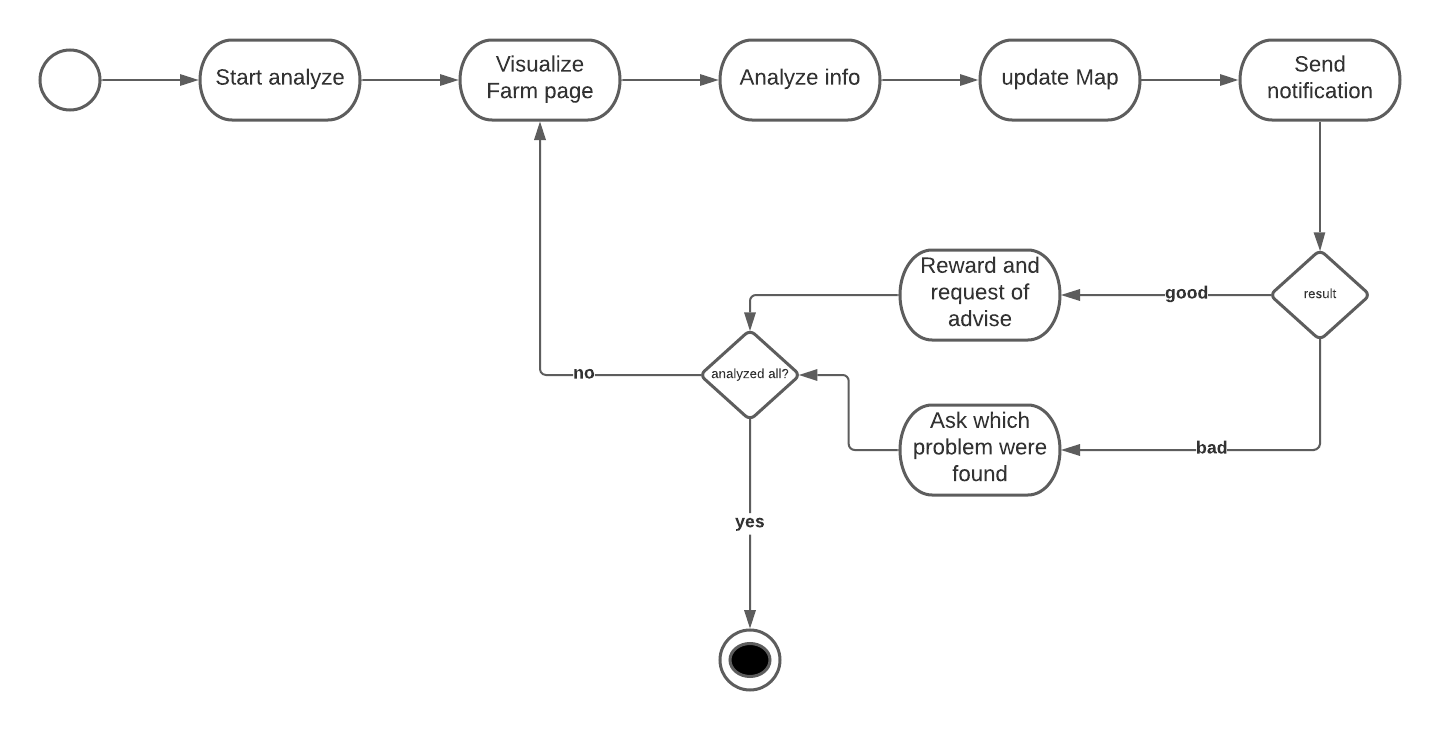
\includegraphics[width=1\textwidth]{images/State chart 2.png}
        \caption{Analysis of farmers.}
        \label{fig:state2}
        \end{center}
    \end{figure}

    \item \textbf{Request of help from a farmer}
    \item The diagram represented in Figure \ref{fig:state3} shows the events that takes place 
    when a farmer sends a request of help. It can happen by writing a message in the forum 
    or by sending a request through a form in the homepage.
    \begin{figure}[H]
        \begin{center}
        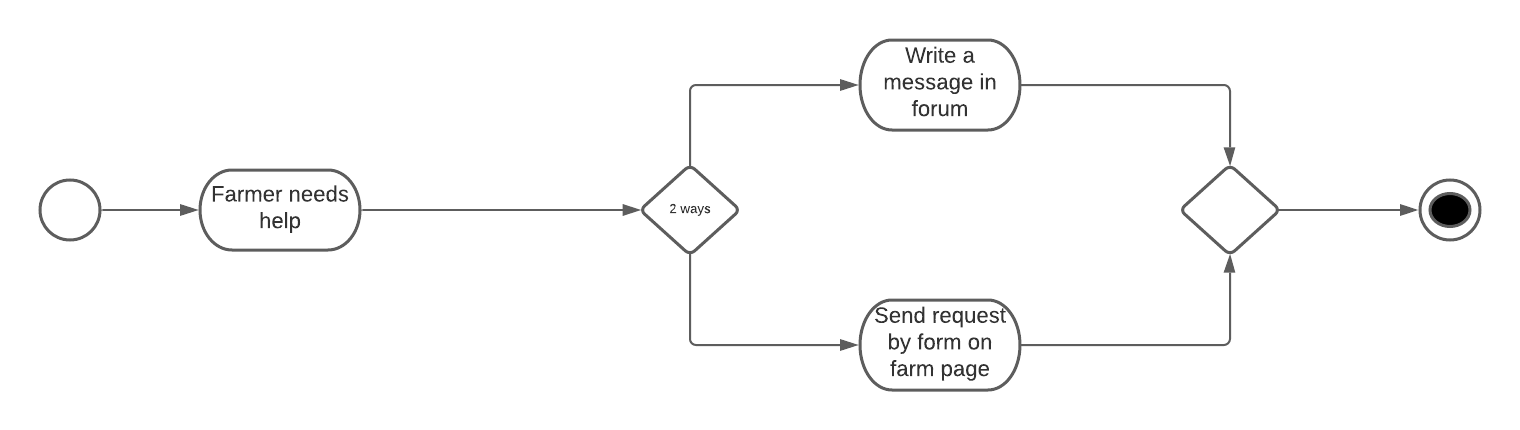
\includegraphics[width=1\textwidth]{images/State chart 3.png}
        \caption{Request of help.}
        \label{fig:state3}
        \end{center}
    \end{figure}
\end{enumerate}
\newpage
\subsection{Product Functions}\label{subsection:2.2}
This section provides a summary of the main features and 
functions offered by the software regarding
the goals already described in section ~\ref{section:1.1.1}

In the following description it is important to highlight that both
the policy makers and the farmers must be logged in.

\subsubsection{Farmers insert data} 
This functionality is accessible to all farmers. 
The application provides a form in which the farmer can easily insert data of his/her production.
The form is easy to fill in, in order to complete it the farmer need to indicate:
\begin{itemize}
    \item the \textbf{type of product}
    \item the \textbf{amount} producted of the selected type
    \item the \textbf{date} relative to the date of the production
\end{itemize}
If the farmer needs to add more than one type of product, 
he/she can fill in the form multiple times.
After completing the form the user is redirected to the homepage and the policy makers 
can see the updated data.
This functionality can be done more than once a day since the farmer can select the date, 
so it is possible for him to insert data of past days too.
This operation can be repeated more than once a day since the farmer can select the date, so it is possible for him/her to insert data of past days too.



\subsubsection{Farmers visualize data}
This functionality lets the farmer visualize all the data 
acquired from the system. The farmer can visualize all data on his homepage.\\
The application shows:
\begin{itemize}
    \item meteorological  short-term and long-term forecast
    \item amount of water used by the farmer
    \item humidity of soil 
    \item personalized suggestions concerning specific crops to plant or specific 
    fertilizers to use – based on their location and type of production
\end{itemize}

\textbf{Should I say why he needs to visualize this data or how he uses it}


This functionality is always up to date, and does not need 
any input from the farmer.
It is used by the farmer only to have a general view of 
his farm and on how he could improve the productivity of his farm.



\subsubsection{Identify how farmers are performing}
The main features of the policy makers is to evaluate the work of each Farmer. 
In order to do that, they periodically analyze each farm page: 
the system allows them to visualize all the data in those pages 
(but not to modify it).
The analysis takes place twice a month.
With this analysis they classify the workers in two different way:
\begin{itemize}
    \item GOOD farmer : those how have been able to produce a significant amount of product with low resources, despite bad weather in that period.
    \item BAD farmer : those who did not produce much.
\end{itemize}
Policy makers inform each farmer the result they have achieved with a notification: 
\begin{itemize}
    \item GOOD farmers receive a special 
    incentive, and also a request to submit 
    from their personal web page some advice that could be useful to the others. 
    \item To BAD farmers is asked to submit an explicit request of help specifying the problems they had.
\end{itemize}
The system has a specific web page that allows all 
the users to look at a map of the area in which are 
specified all the farms. It is also shown if the farm's owner has performed 
a good job in that period.
At the end of each analysis the policy makers 
update the map (they are the only ones that are able to modify it).


\subsubsection{Interaction between farmers}
This functionality permits the farmers to comunicate with each other. 
The application has a specific web page were the farmers can send messages 
whenever they want.
If a farmer has an issue, before submitting a formal request of help to 
the policy makers 
by their home page, he can ask informally an advice by sending a message 
in the Forum.
It is not necessary to be a good farmer in order to answer someone elses 
message. All the messages are visible to everyone and 24h. 
Since it is an online application an internet connection is required 
to read or write on this page.

%---------------------------------------------------------------------------%
\subsection{User Characteristics}
Dream has two different customers that need to be 
distinguished in order to provide the various 
features specified in subsection ~\ref{subsection:2.2}.

\subsubsection{Farmer}
\begin{itemize}
    \renewcommand\labelitemi{--}
    \item Can register on Dream in order to be recognized as farmer
    \item Must log in on the website to use the services offered
    \item Can discuss with other farmers
    \item Is able to insert data about their daily production
    \item Can ask for help to other farmers or to policy makers
    \item Can retrieve data regarding weather forecast, water irrigation system or humidity of soil
    \item Can look for advice of several products
    \item Can check whether their performance is identified as good or bad
\end{itemize}

\subsubsection{Policy Maker}

\begin{itemize}
    \renewcommand\labelitemi{--}
    \item Already has the credential to access to the system
    \item Must login to Dream to benefit of its services
    \item Can look all farms' pages
    \item Can update the map
    \item Can send suggestions to whom explicitly notices a problem
    \item Can send notifications to the farmers
    \item Decides the value of the incentive for the good farmers
    \item Evaluates the performance of the farmers
\end{itemize}


\subsection{Domain Assumptions, Dependencies and Constraints}
This subsection focuses on what it is assumed in order for our system to offer the services as expected.
Moreover it focuses on the limitations that the system could face.

\subsubsection{Domain Assumptions}
\textbf{DA1} In order to access the system users need to have Internet connection.\\
\textbf{DA2} Farmers always insert correct data on their production activity.\\
\textbf{DA3} Data from sensors is always correct.\\
\textbf{DA4} Date and Time on the system are always correct.\\
\textbf{DA5} The position of the Farm is always correct.\\
\textbf{DA6} Internet connection works always without errors.\\
\textbf{DA7} Meteorological data is accurate.\\
\textbf{DA8} Every farm has a different position.\\
\textbf{DA9} Each farm belongs to exacly one farmer.\\
\textbf{DA10} Discussion on the forum are related only to the farm activity.\\
\textbf{DA11} Formal request of help must be related to a farmer's own production.\\
\textbf{DA12} Advice on a product must be given by a farmer that produces the same type.\\
\textbf{DA13} Performances of farmers are always identified correctly.\\
\textbf{DA14} Farmers can insert data more than once a day.\\
\textbf{DA15} The email and farm's name must be unique.\\
\textbf{DA16} Policy Makers have a given code and password to access the system.\\
\textbf{DA17} All farmers that sign up own a real farm in Telengana.\\
\textbf{DA18} The special incentive that the farmers received for their good work, is used on stuff related to their production. \\


\subsubsection{Constraints}

%-----------------------------------------------------------%
\newpage
\section{Specific Requirements}
\subsubsection{External Interface Requirements}
This section of the document gives a clear description of all the requirments that the system needs in order to performe all 
the functionalities described in section \ref{subsection:2.2}.

\subsubsection{User Interfaces}
The following mockups of the web application provide a first idea on how the features of the system are offered to the users. 
Moreover it gives a real perpespective of how the users interact with the system. 
The Design Document (reference) provides a thorough and detailed description of the features represented in each mockup.

\begin{figure}[H]
    \begin{center}
    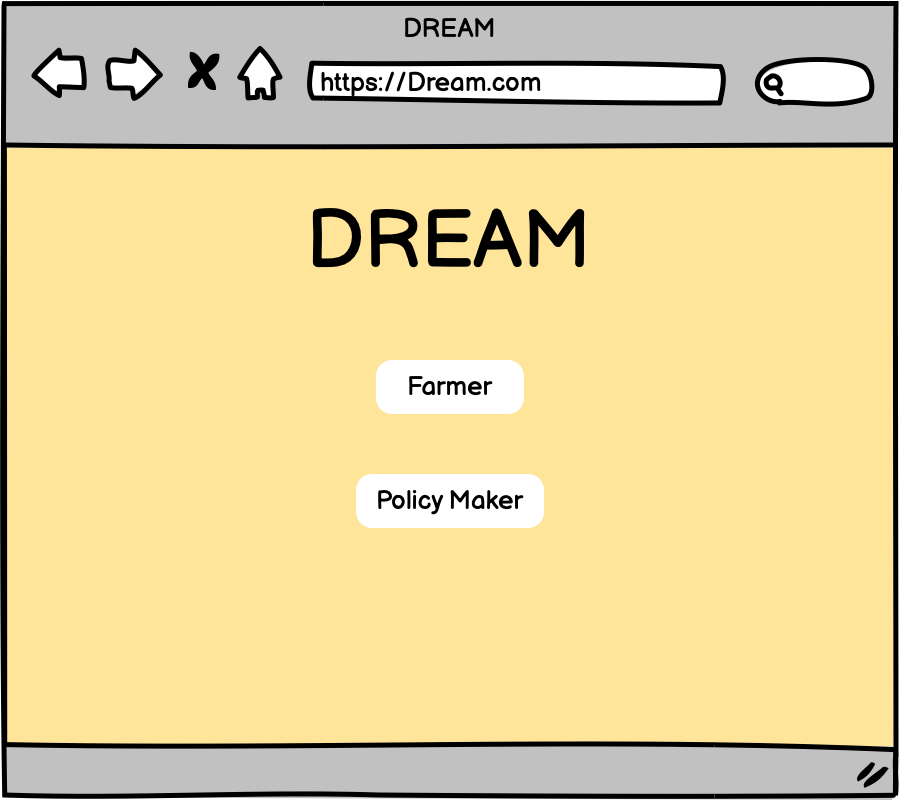
\includegraphics[width=0.6\textwidth]{mockups/Dream.png}
    \caption{\emph{DREAM} Web page}
    \label{fig:webPage}
    \end{center}
\end{figure}
 
\begin{figure}[ht!]
    \begin{minipage}{0.5\textwidth}
        \centering
        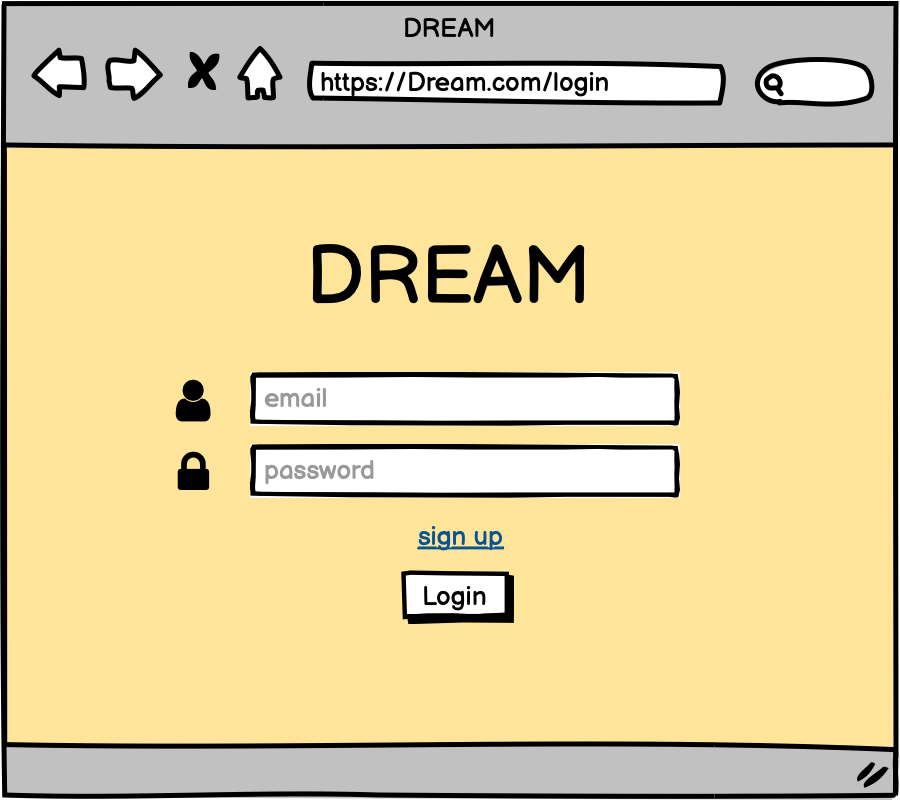
\includegraphics[width=1\textwidth]{mockups/FLogIn.png}
        \caption{\emph{Farmer Log in} Web page}
        \label{fig:mockupLogin}
    \end{minipage}\hfill
    \begin{minipage}{0.5\textwidth}
        \centering
        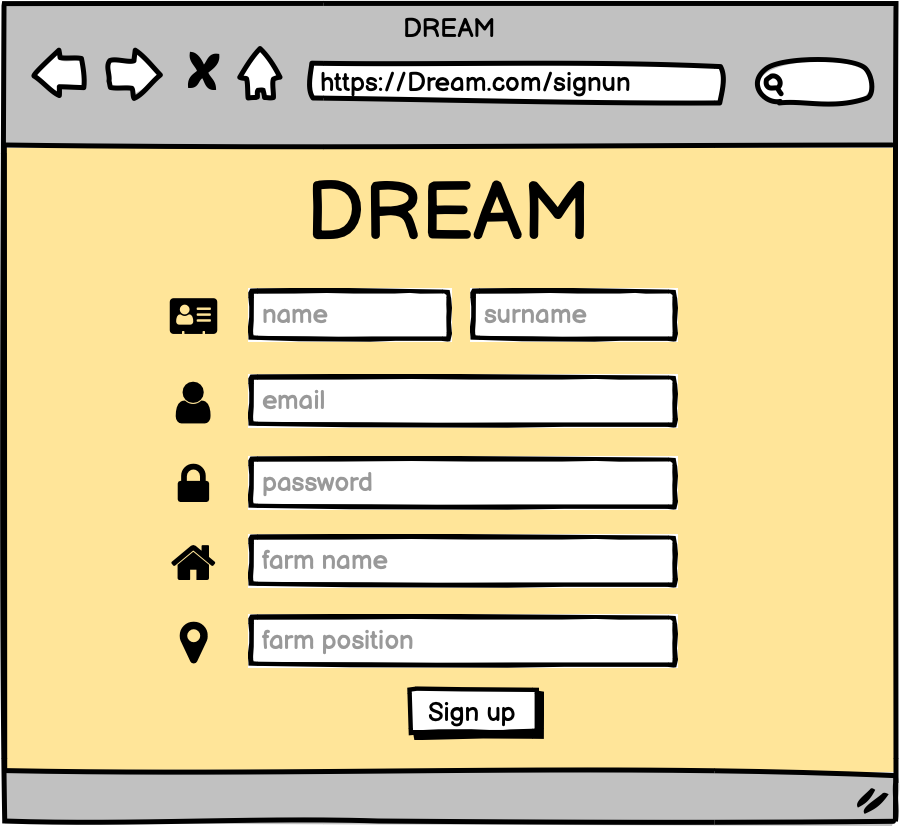
\includegraphics[width=1\textwidth]{mockups/SignUp.png}
        \caption{\emph{Farmer Sign up} Web page}
        \label{fig:smockupSignUp}
    \end{minipage}
\end{figure}

\begin{figure}[H]
    \begin{center}
    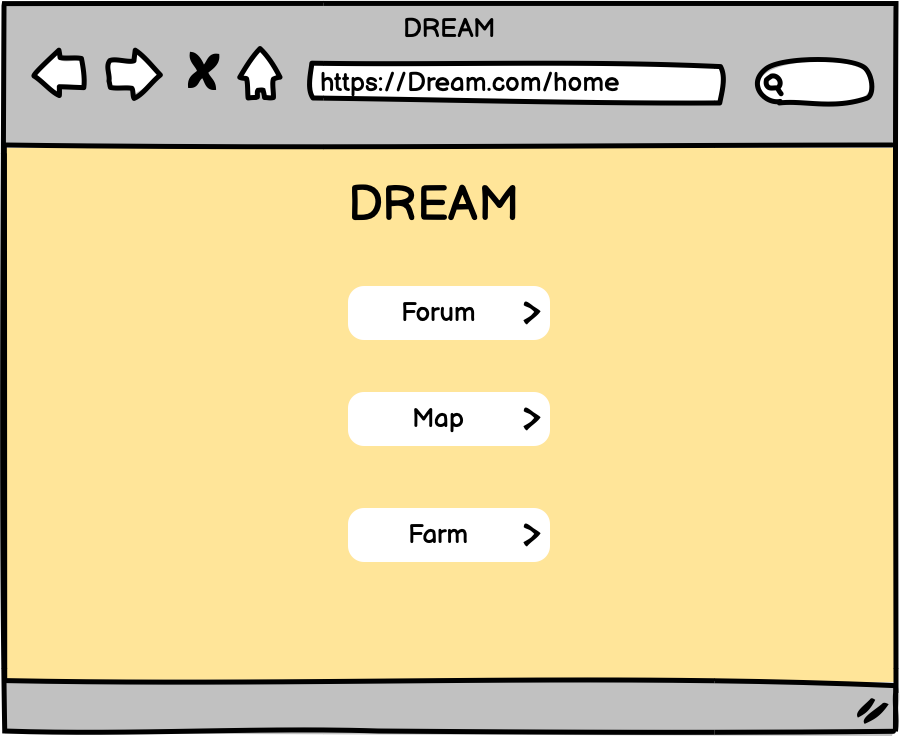
\includegraphics[width=0.6\textwidth]{mockups/FHome.png}
    \caption{\emph{Farmer} Home page}
    \label{fig:homepage}
    \end{center}
\end{figure}

\begin{figure}[H]
    \begin{center}
    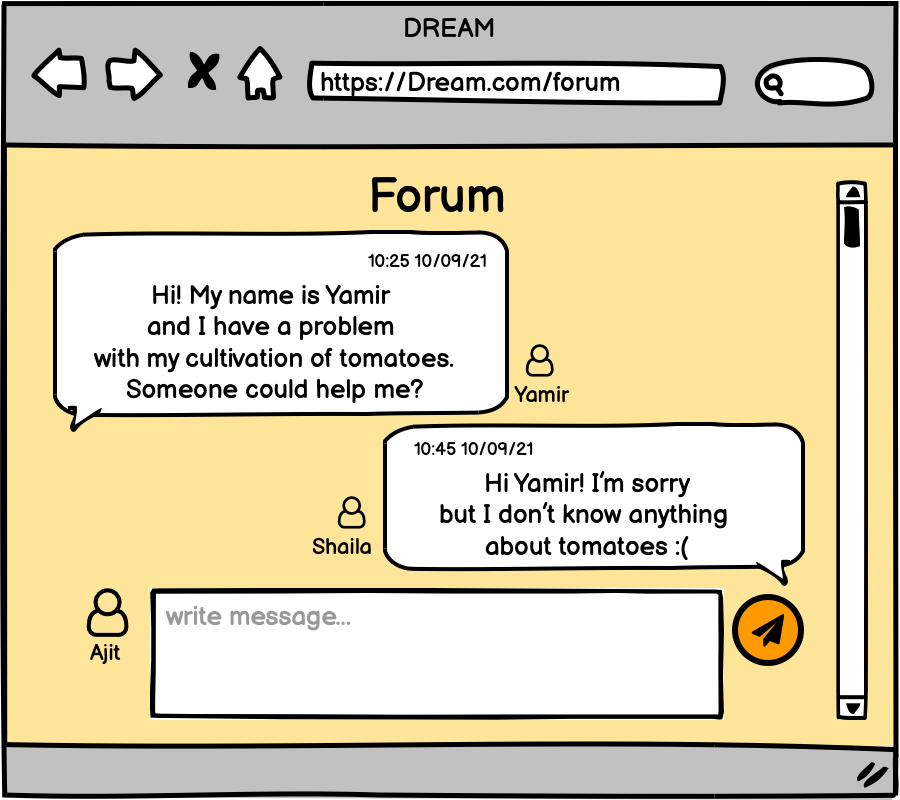
\includegraphics[width=0.7\textwidth]{mockups/Forum.png}
    \caption{\emph{Forum} Web page}
    \label{fig:forum}
    \end{center}
\end{figure}

\begin{figure}[H]
    \begin{center}
    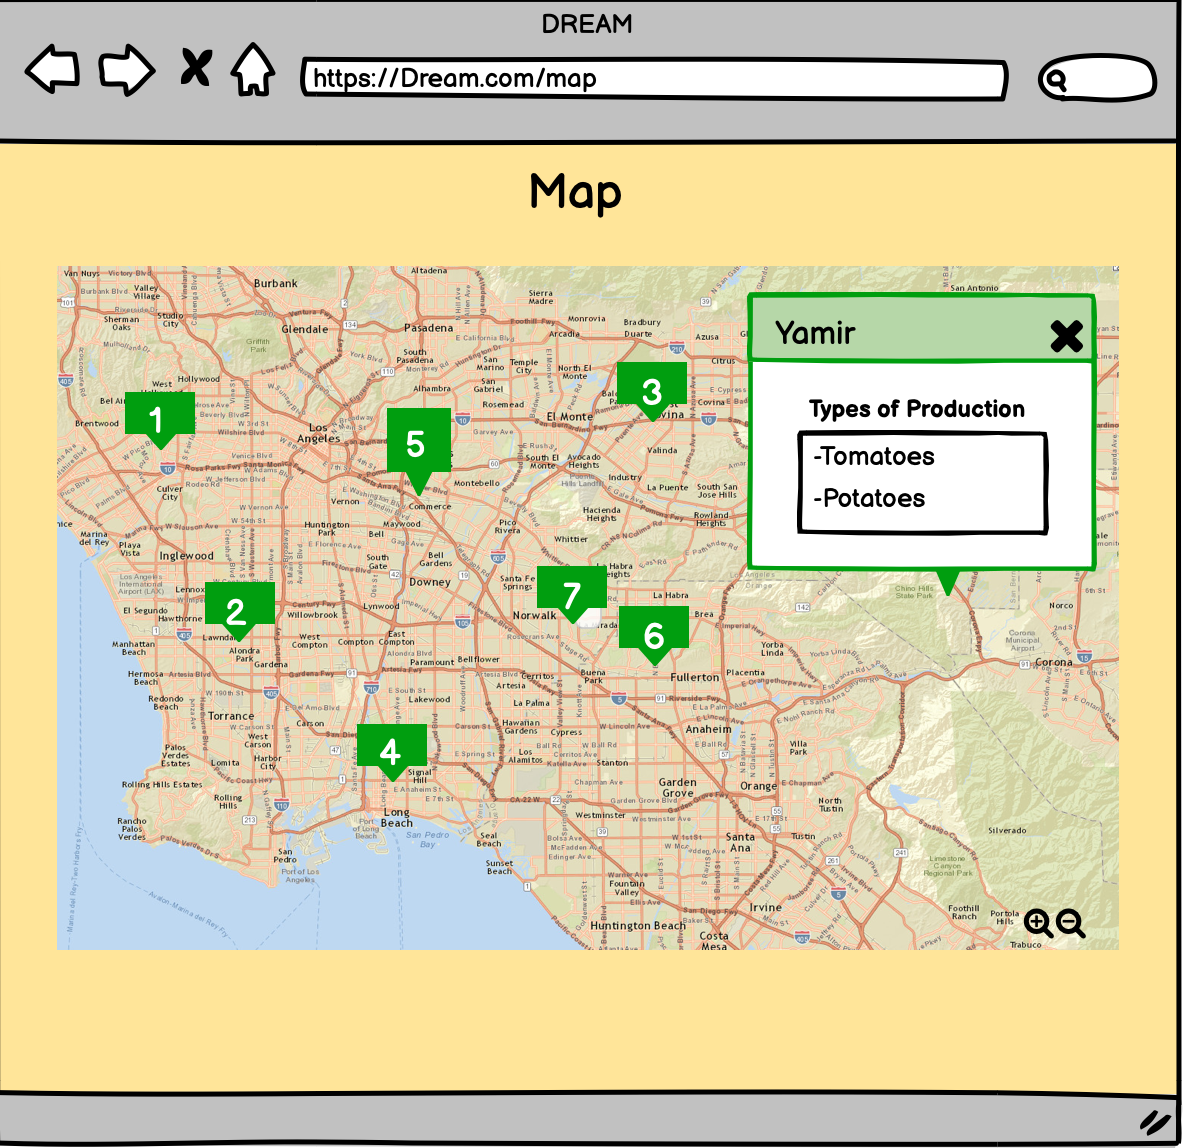
\includegraphics[width=0.7\textwidth]{mockups/FMap.png}
    \caption{\emph{Farmer } Map page}
    \label{fig:farmerMap}
    \end{center}
\end{figure}

\begin{figure}[H]
    \begin{center}
    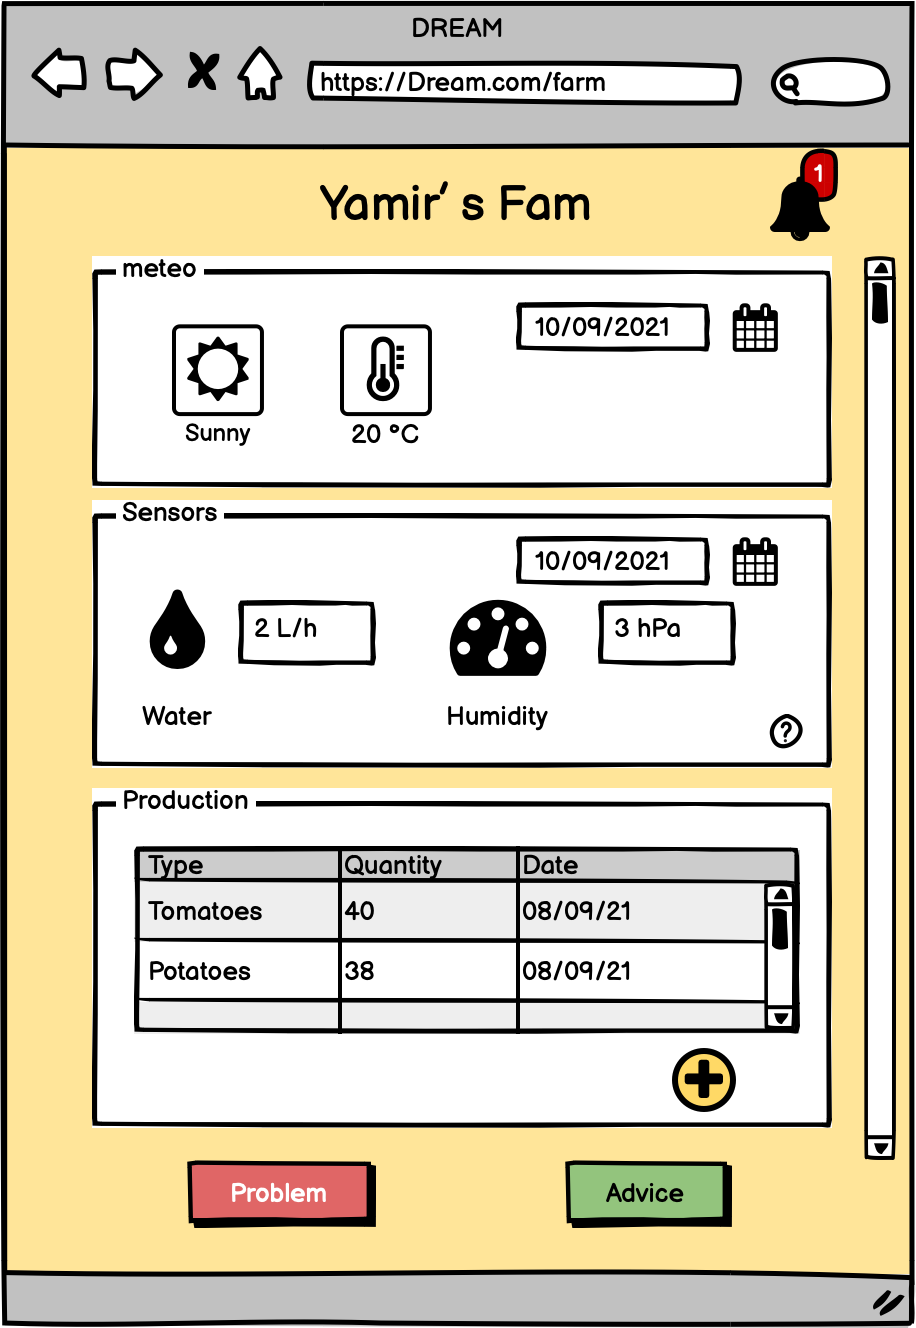
\includegraphics[width=0.7\textwidth]{mockups/FFarm.png}
    \caption{\emph{Farmer's} Farm page}
    \label{fig:FarmPage}
    \end{center}
\end{figure}

\begin{figure}[H]
    \begin{center}
    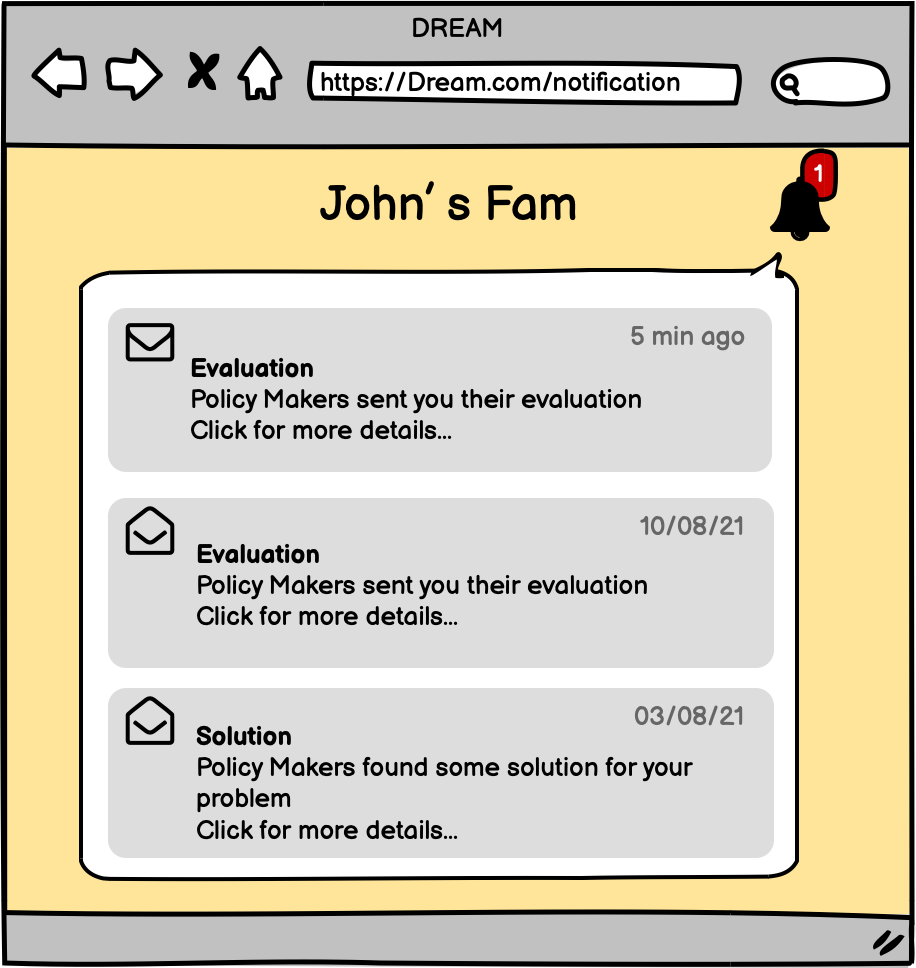
\includegraphics[width=0.7\textwidth]{mockups/Notifications.png}
    \caption{\emph{Farmer's notifications list}}
    \label{fig:notificationList}
    \end{center}
\end{figure}

\begin{figure}[H]
    \begin{center}
    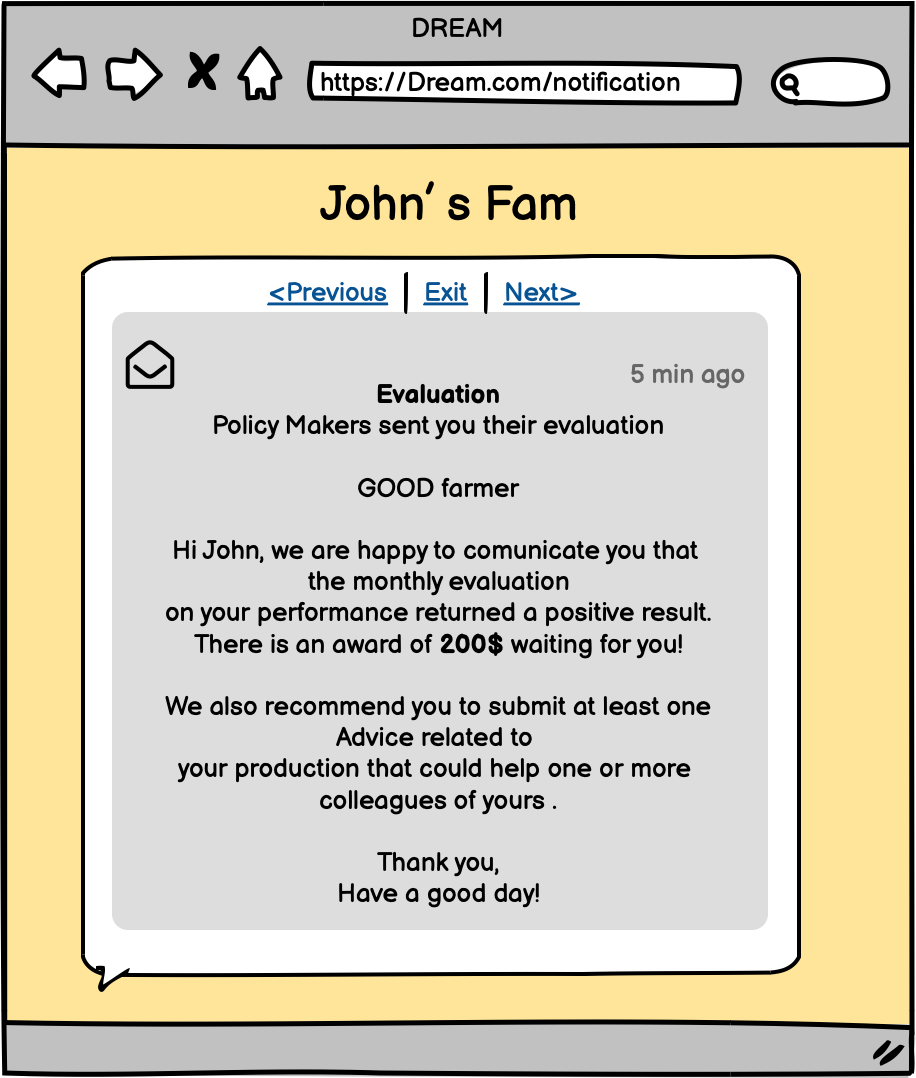
\includegraphics[width=0.7\textwidth]{mockups/Notification.png}
    \caption{\emph{Farmer's single notification}}
    \label{fig:singleNotification}
    \end{center}
\end{figure}

\begin{figure}[H]
    \begin{center}
    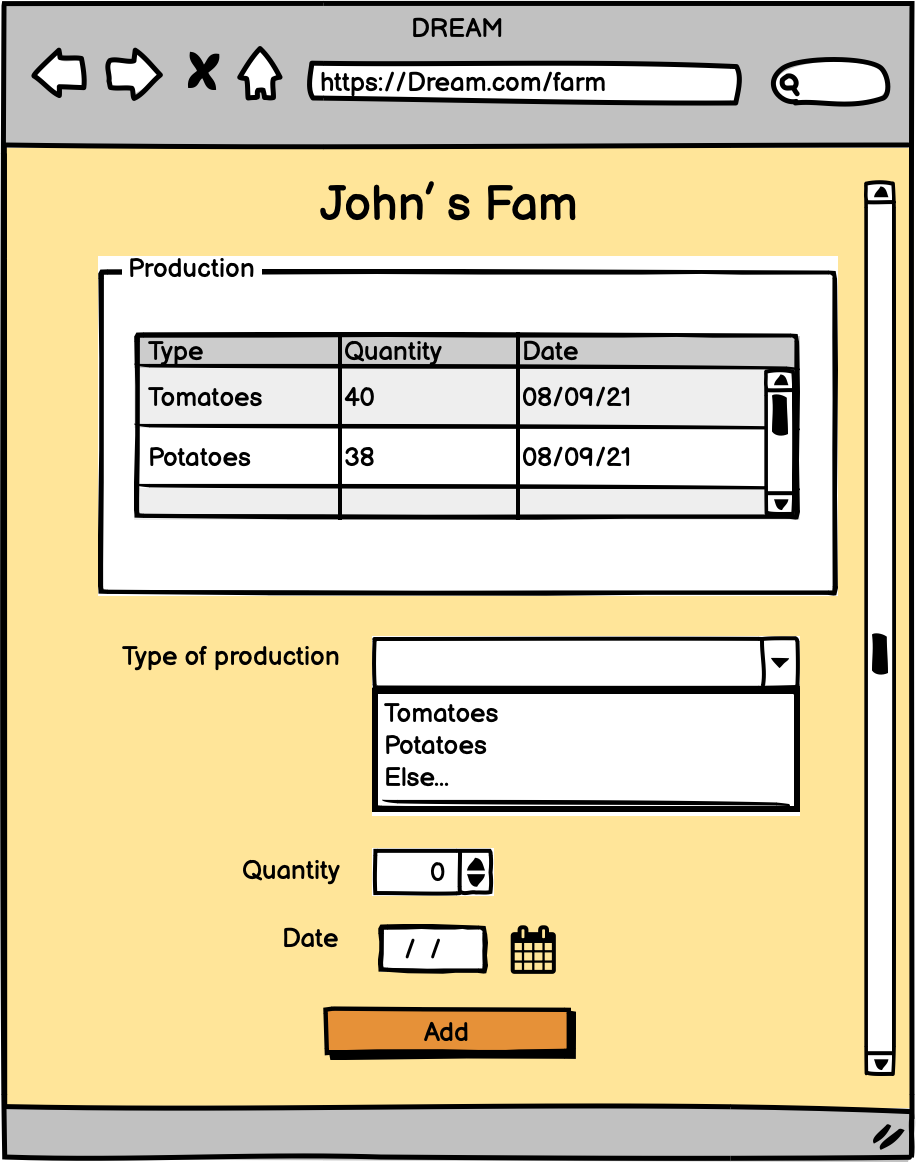
\includegraphics[width=0.7\textwidth]{mockups/AddData.png}
    \caption{\emph{Farmer add data} Web page}
    \label{fig:addData}
    \end{center}
\end{figure}

\begin{figure}[H]
    \begin{center}
    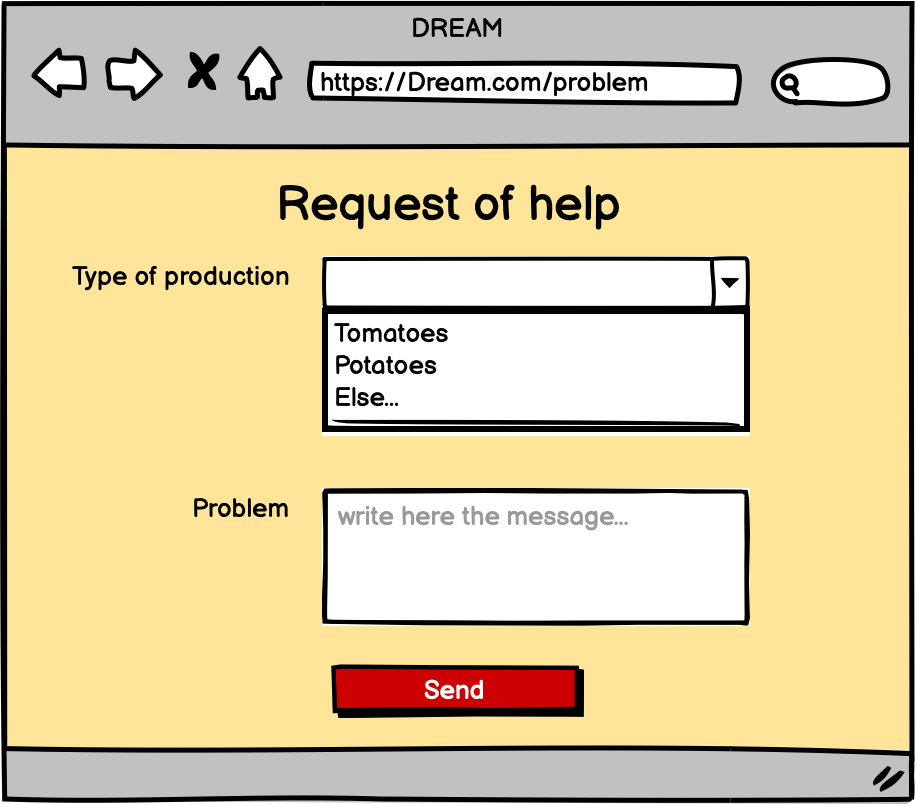
\includegraphics[width=0.7\textwidth]{mockups/Help.png}
    \caption{\emph{Farmer send request of help} Web page}
    \label{fig:helpRequest}
    \end{center}
\end{figure}

\begin{figure}[H]
    \begin{center}
    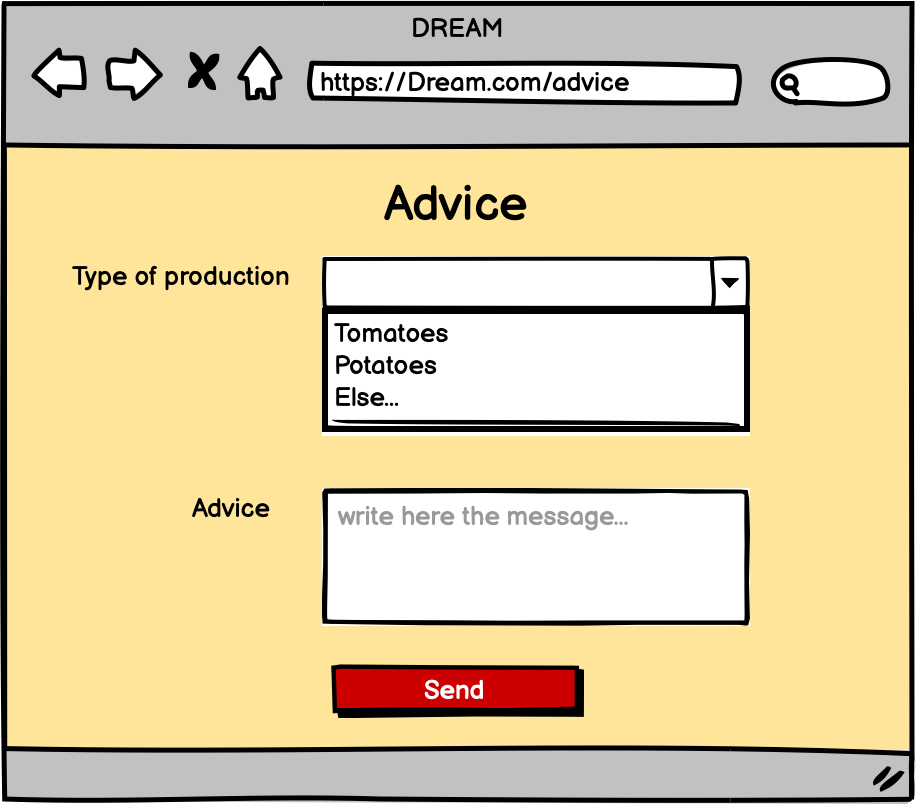
\includegraphics[width=0.7\textwidth]{mockups/Advice.png}
    \caption{\emph{Farmer submit advice} Web page}
    \label{fig:submit advice}
    \end{center}
\end{figure}

\begin{figure}[H]
    \begin{center}
    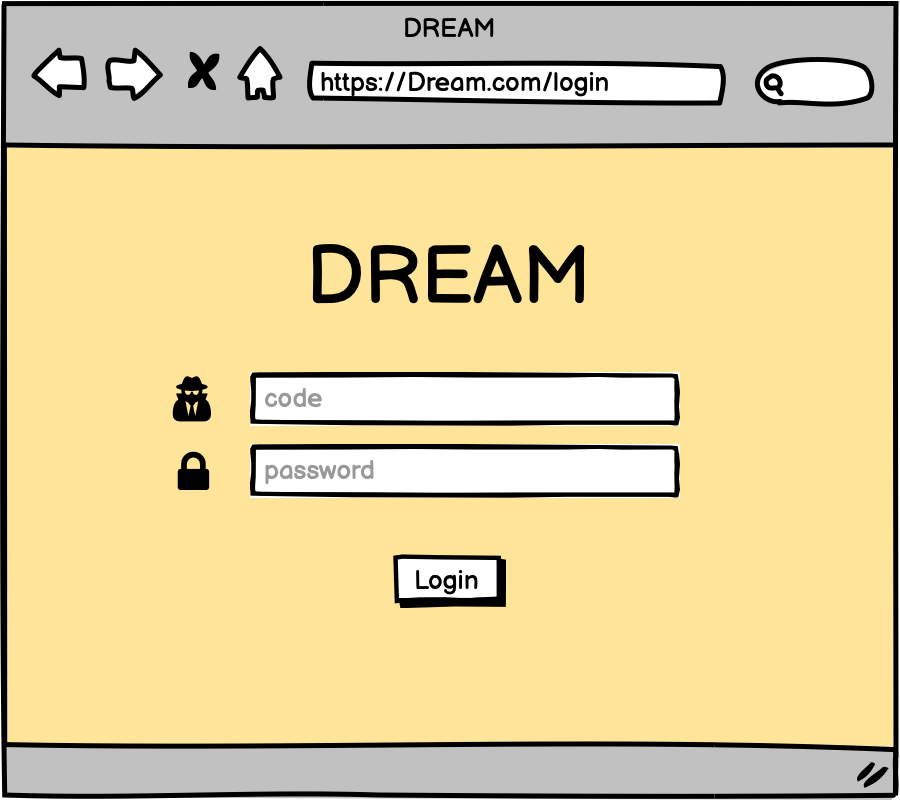
\includegraphics[width=0.7\textwidth]{mockups/PMLogIn.png}
    \caption{\emph{Policy Maker Log in} Web page}
    \label{fig:PMlogin}
    \end{center}
\end{figure}

\begin{figure}[H]
    \begin{center}
    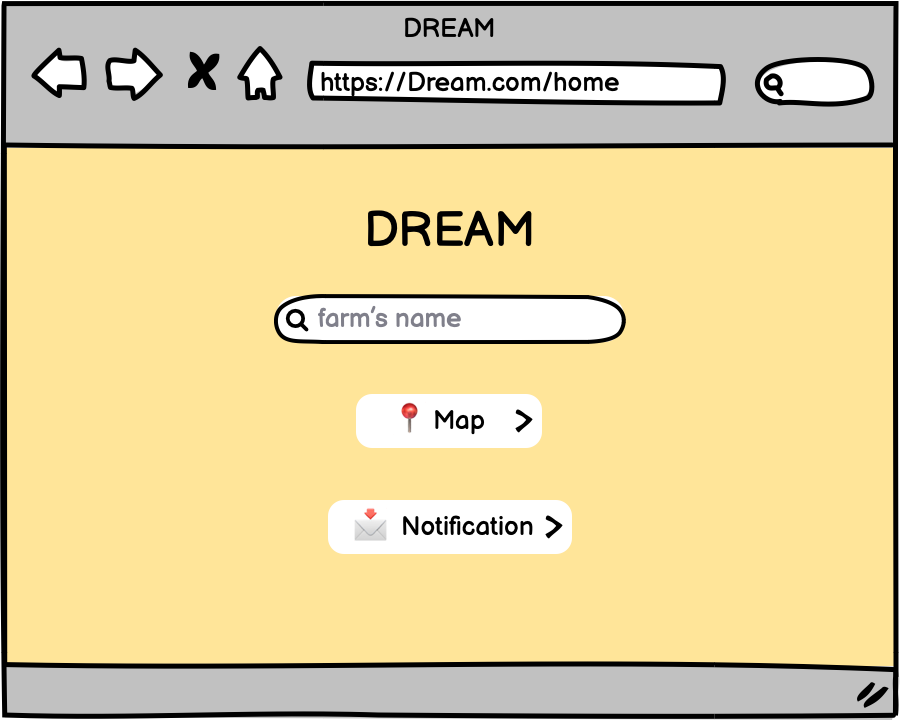
\includegraphics[width=0.7\textwidth]{mockups/PMHome.png}
    \caption{\emph{Policy Maker} Home page}
    \label{fig:PMhomepage}
    \end{center}
\end{figure}

\begin{figure}[H]
    \begin{center}
    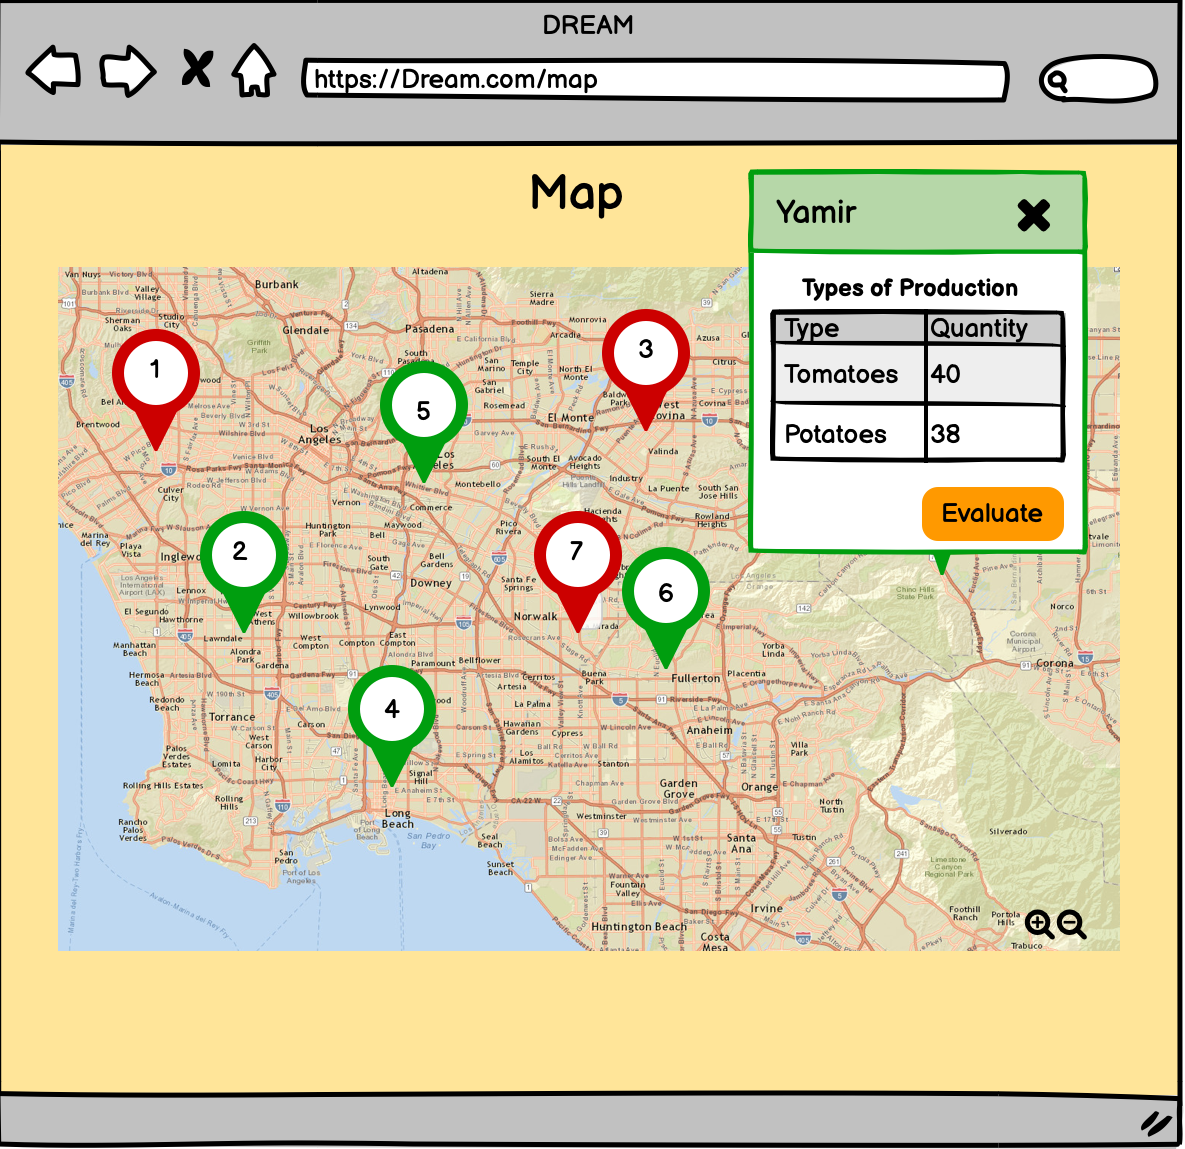
\includegraphics[width=0.7\textwidth]{mockups/PMMap.png}
    \caption{\emph{Policy Maker} Map page}
    \label{fig:PMmap}
    \end{center}
\end{figure}

\begin{figure}[H]
    \begin{center}
    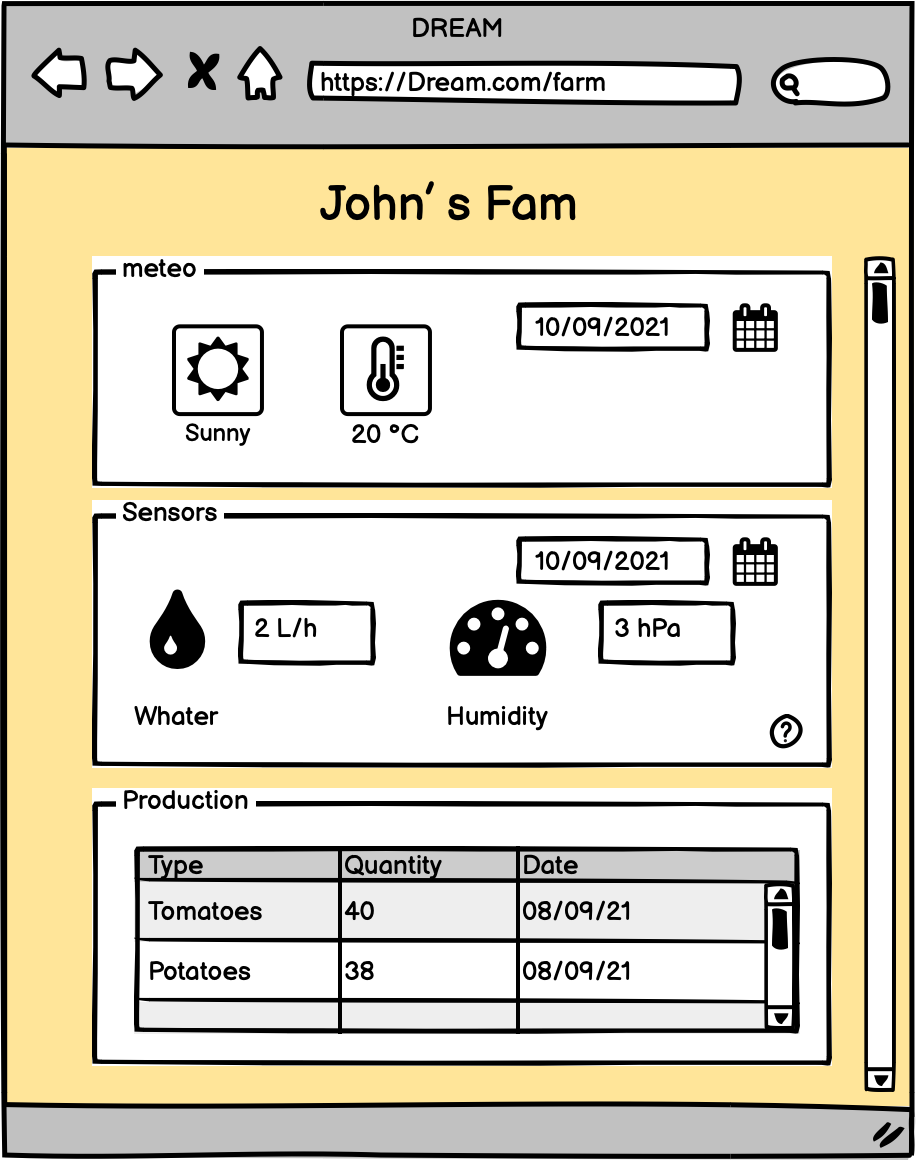
\includegraphics[width=0.7\textwidth]{mockups/PMFarm.png}
    \caption{\emph{Policy Maker} Farm's page visualization}
    \label{fig:PMFarmPage}
    \end{center}
\end{figure}

\begin{figure}[H]
    \begin{center}
    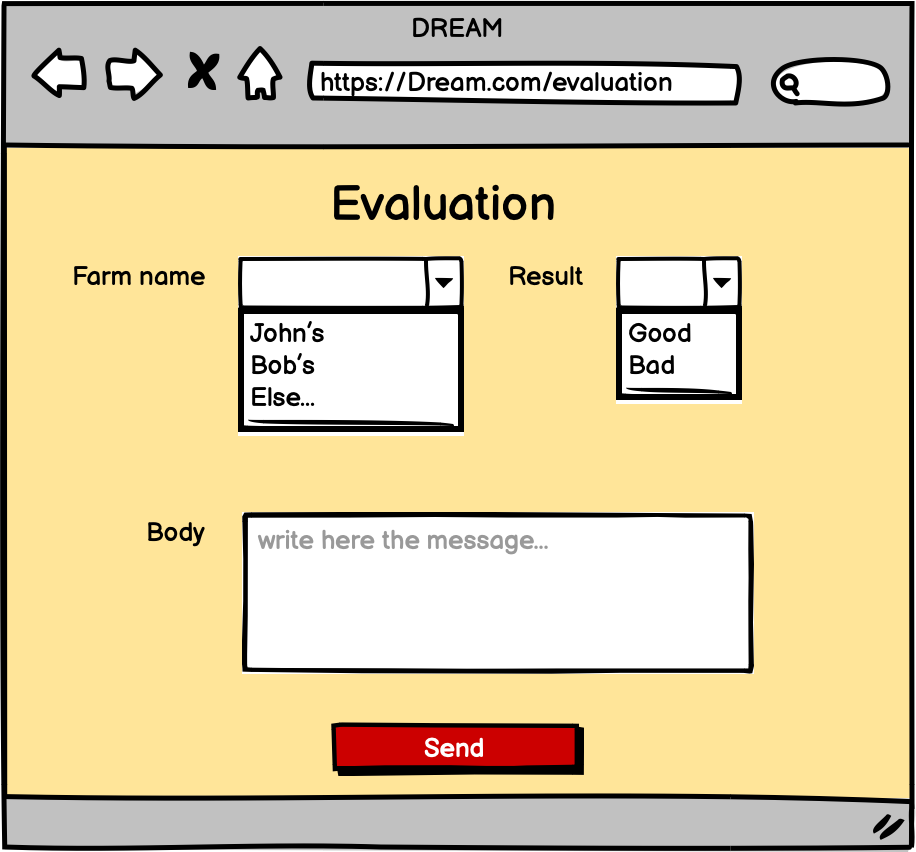
\includegraphics[width=0.7\textwidth]{mockups/Evaluation.png}
    \caption{\emph{Policy Maker} evaluation page}
    \label{fig:PMevaluation}
    \end{center}
\end{figure}

\begin{figure}[H]
    \begin{center}
    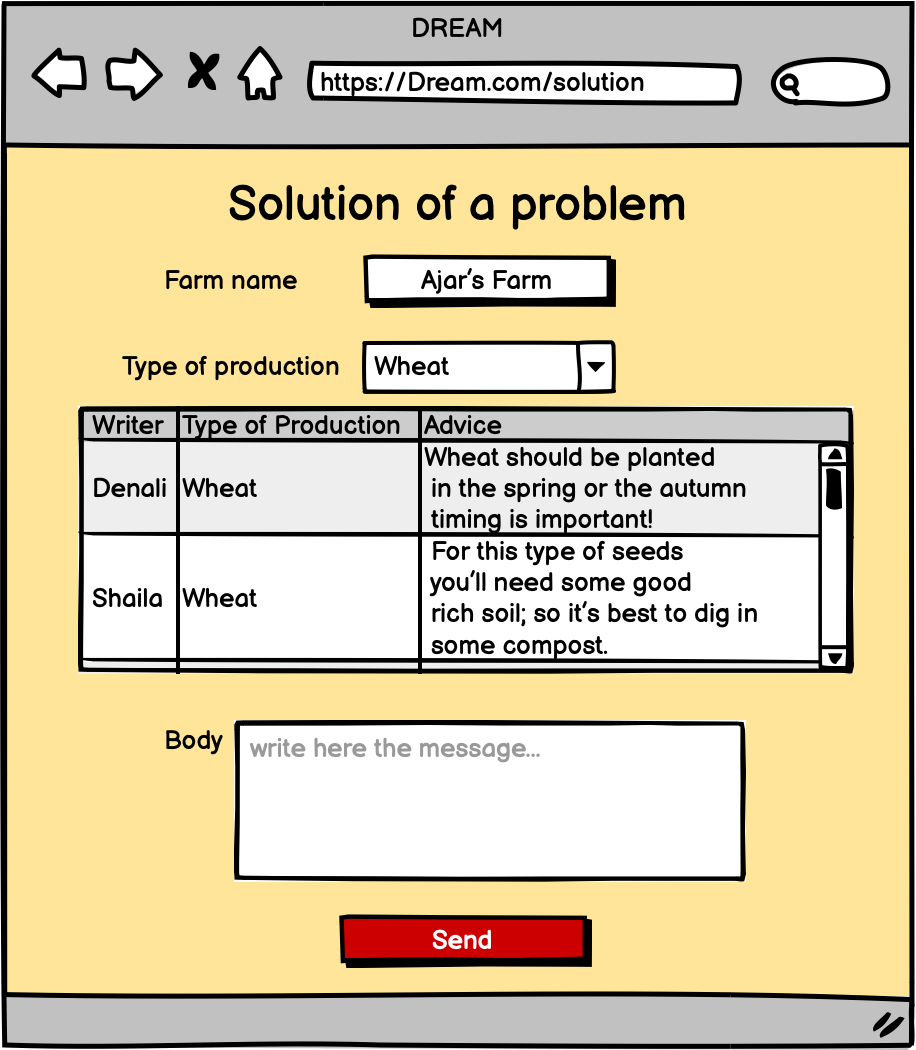
\includegraphics[width=0.7\textwidth]{mockups/Solution.png}
    \caption{\emph{Policy Maker} send solution page}
    \label{fig:PMsolution}
    \end{center}
\end{figure}

\subsubsection{Hardware Interfaces}
The application does not need any specific hardware requirements. 

\subsubsection{Software Interfaces}
The web app requires a computer with a web browser installed and connected to 
The system has to rely on a DBMS API. It allows the management of all the data the system 
needs in order to provide its functionalities, described in subsection ~\ref{subsection:2.2}.

\subsubsection{Communication Interfaces}
All the communications between users and Dream website are made via HTTPS.

\newpage

\subsection{Functional Requirements}
\subsubsection{Use Case Diagram}
\begin{figure}[H]
    \begin{center}
    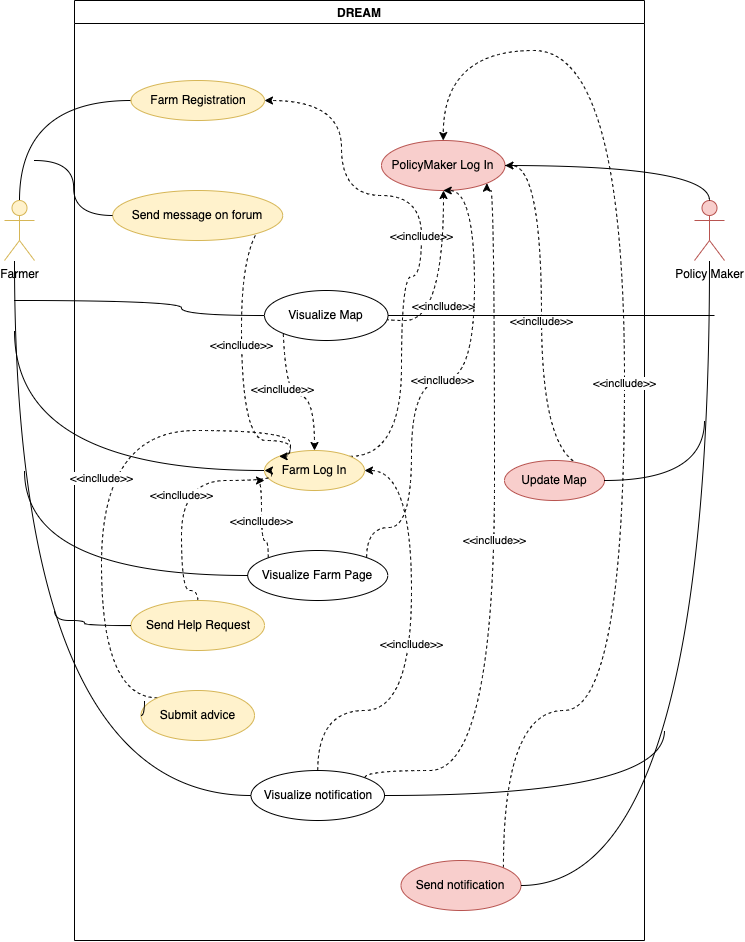
\includegraphics[width=1\textwidth]{images/useCaseDiag.drawio.png}
    \caption{Use Case diagram.}
    \label{fig:state9}
    \end{center}
\end{figure}
\subsubsection{Use Cases Description ad Sequence Diagram}
\begin{enumerate}
    \item \textbf{Farmer Registration} 
        \begin{longtable}{p{0.26\linewidth}p{0.75\linewidth}}
            \toprule
            \textbf{Name} & \textbf{Farmer Registration} \\
            \midrule
            \textbf{Actors} & Farmer \\
            \midrule
            \textbf{Entry conditions} & The web application has started\\
            \midrule
            \textbf{Flow of events} & 
            \begin{enumerate}
                \item The farmer wants to sign up
                \item The farmer inserts email, name, password, farm's name and farm's position 
                \item The farmer clicks submit
                \item The system checks if email is unique and if all the form is correctly fill up 
                \item The system inserts the information in the data base
            \end{enumerate} \\
            \midrule
            \textbf{Exit conditions} & The farmer is signed up\\
            \midrule
            \textbf{Exceptions} & 
            \begin{itemize}
                \item If the farmer did not insert data correctly the system will send an alert and let the user do that again
                \item If the email is already present in the database the system will send an alert saying that the email already exists
            \end{itemize} \\
            \bottomrule
            \caption{\emph{Farmer Registration} use case description}
        \end{longtable}
        
            \begin{figure}[H]
                \begin{center}
                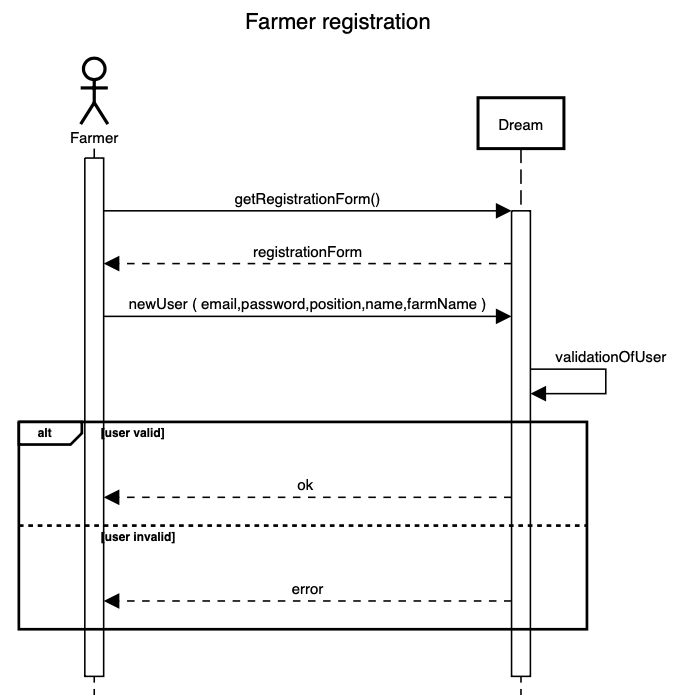
\includegraphics[width=0.7\textwidth]{sequence/FarmerRegistration.png}
                \caption{\emph{Farmer Registration} sequence diagram}
                \label{fig:sequence1}
                \end{center}
            \end{figure}

        \item \textbf{Farmer Login}
        \begin{longtable}{p{0.26\linewidth}p{0.75\linewidth}}
            \toprule
            \textbf{Name} & \textbf{Farmer Login} \\
            \midrule
            \textbf{Actors} & Farmer \\
            \midrule
            \textbf{Entry conditions} & The web application has started\\
            \midrule
            \textbf{Flow of events} & 
            \begin{enumerate}
                \item The farmer wants to log in
                \item The farmer inserts email and password
                \item The farmer clicks submit
                \item The system checks if the credentials are correct
                \item The system notifies the farmer about the correct login
            \end{enumerate} \\
            \midrule
            \textbf{Exit conditions} & The farmer has logged in\\
            \midrule
            \textbf{Exceptions} & 
            \begin{itemize}
                \item If the system does not recognize the email it will send and alert to the farmer saying that the email inserted is wrong
                \item If the password is not correct the system will notify the farmer
            \end{itemize} \\
            \bottomrule
            \caption{\emph{Farmer Login} use case description}
        \end{longtable}
        
        \begin{figure}[H]
        \begin{center}
        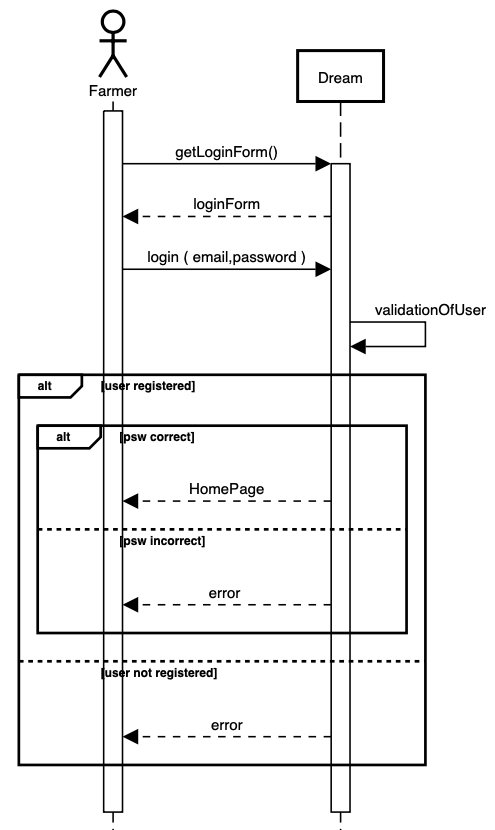
\includegraphics[width=0.5\textwidth]{sequence/FarmerLogin.png}
        \caption{\emph{Farmer Login} sequence diagram}
        \label{fig:sequence2}
        \end{center}
        \end{figure}


        \item Farmer send a message on the Forum
        \item \begin{longtable}{p{0.26\linewidth}p{0.75\linewidth}}
            \toprule
            \textbf{Name} & \textbf{Farmer sends a message on the forum} \\
            \midrule
            \textbf{Actors} & Farmer \\
            \midrule
            \textbf{Entry conditions} & The farmer has logged in\\
            \midrule
            \textbf{Flow of events} & 
            \begin{enumerate}
                \item The farmer wants to send a message
                \item The farmer clicks on forum button
                \item The system send the ser to the forum page
                \item The farmer inserts the message 
                \item The farmer clicks on send message
                \item The system inserts the message into the database 
            \end{enumerate} \\
            \midrule
            \textbf{Exit conditions} & The farmer's message is published\\
            \midrule
            \textbf{Exceptions} & 
            \begin{itemize}
                \item If the message body is empty the system shows an error alert
            \end{itemize} \\
            \bottomrule
            \caption{\emph{Farmer message} use case description}
        \end{longtable}
        \begin{figure}[H]
            \begin{center}
            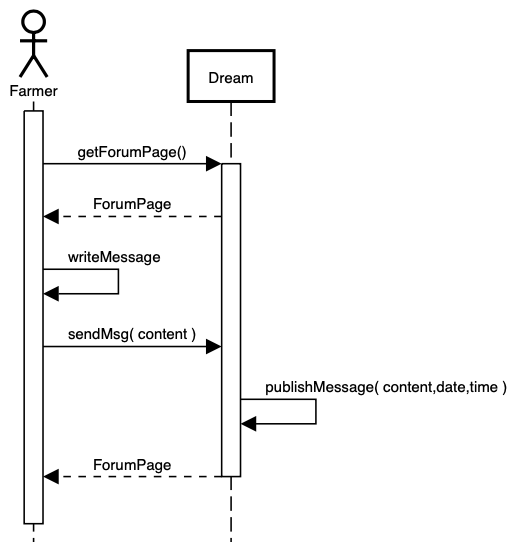
\includegraphics[width=0.6\textwidth]{sequence/messageOnForum.png}
            \caption{\emph{Farmer message} sequence diagram}
            \label{fig:sequence3}
        \end{center}
        \end{figure}

    \item Find a farmer on the Map\\
    \begin{longtable}{p{0.26\linewidth}p{0.75\linewidth}}
        \toprule
        \textbf{Name} & \textbf{Farmer visualizes the map} \\
        \midrule
        \textbf{Actors} & Farmer \\
        \midrule
        \textbf{Entry conditions} & The farmer has logged in\\
        \midrule
        \textbf{Flow of events} & 
        \begin{enumerate}
            \item The farmer wants to visualize the map
            \item The farmer clicks on map button
            \item The system send the farmer to the map page
            \item The farmer visualizes the map and selects a farm
            \item The system retrieves the information about the farm and shows them to the farmer
            \item The farmer visualizes the data about the selected farm
        \end{enumerate} \\
        \midrule
        \textbf{Exit conditions} & The farmer visualized the map\\
        \midrule
        \textbf{Exceptions} & \\
        \bottomrule
        \caption{\emph{Farms' map visualization} use case description}
    \end{longtable}
    \begin{figure}[H]
        \begin{center}
        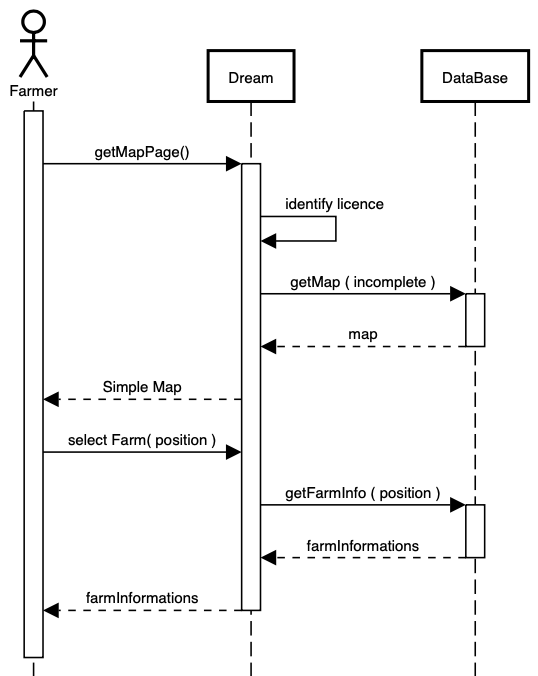
\includegraphics[width=0.45\textwidth]{sequence/VisializeMap.png}
        \caption{\emph{Farms' map visualization} sequence diagram}
        \label{fig:sequence4}
        \end{center}
    \end{figure}
    
    \item Find farm’s information
    \begin{longtable}{p{0.26\linewidth}p{0.75\linewidth}}
        \toprule
        \textbf{Name} & \textbf{Farmer visualizes their own data} \\
        \midrule
        \textbf{Actors} & Farmer \\
        \midrule
        \textbf{Entry conditions} & The farmer has logged in\\
        \midrule
        \textbf{Flow of events} & 
        \begin{enumerate}
            \item The farmer wants to visualize his own page
            \item The farmer clicks on the profile page button
            \item The system retrives the information about the farmer and redirect him to the farmer's farm page
            \item The farmer visualizes his own page
        \end{enumerate} \\
        \midrule
        \textbf{Exit conditions} & The farmer visualizes his own data\\
        \midrule
        \textbf{Exceptions} & 
        \begin{enumerate}
            \item
        \end{enumerate}\\
        \bottomrule
        \caption{\emph{Farm information visualization} use case description}
    \end{longtable}
    \begin{figure}[H]
        \begin{center}
        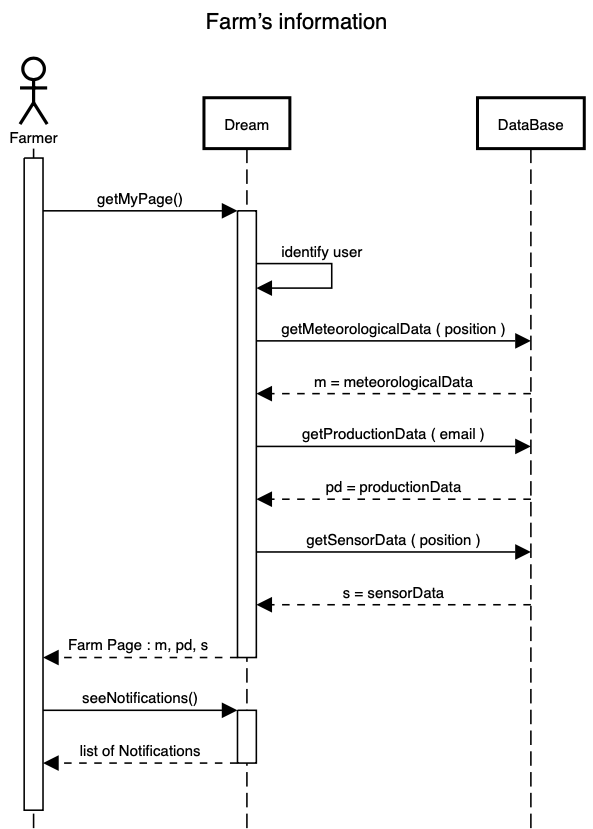
\includegraphics[width=0.7\textwidth]{sequence/FarmInformation.png}
        \caption{\emph{Farm information visualization} sequence diagram}
        \label{fig:sequence5}
        \end{center}
    \end{figure}

    \item Submit a request of help\\
    \textbf{I put only the case of a forml request to the Policy Maker (button on Farm Page) if you want we can create 2 "secion" (alt) one with this formal request and one sending a message on Forum (but is yet specified in 3)}
    \begin{longtable}{p{0.26\linewidth}p{0.75\linewidth}}
        \toprule
        \textbf{Name} & \textbf{Farmer submit a request of help} \\
        \midrule
        \textbf{Actors} & Farmer \\
        \midrule
        \textbf{Entry conditions} & The farmer has logged in\\
        \midrule
        \textbf{Flow of events} & 
        \begin{enumerate}
            \item The farmer wants to ask for help
            \item The farmer clicks on his own page button
            \item The farmer clicks on Help button
            \item The farmer chooses the type of production on which he had problems
            \item The farmer fills the form specifying the problem
            \item The farmer clicks on the submit button and sends the message
            \item The system sends the notification to the Policy Makers
            \item The system notifies the farmer that the operation went succesfully
            \item The system returns a list of advices retrieved from the database about the type of production selected
        \end{enumerate} \\
        \midrule
        \textbf{Exit conditions} & The help request is sent to the Policy Makers\\
        \midrule
        \textbf{Exceptions} & 
        \begin{itemize}
            \item If no type of production is selected the system notifies the farmer and waits for him to insert it
            \item If the request body is empty the system notifies the farmer and waits for him to fill it in
        \end{itemize}\\
        \bottomrule
        \caption{\emph{Farmer ask for help} use case description}
    \end{longtable}
    \begin{figure}[H]
        \begin{center}
        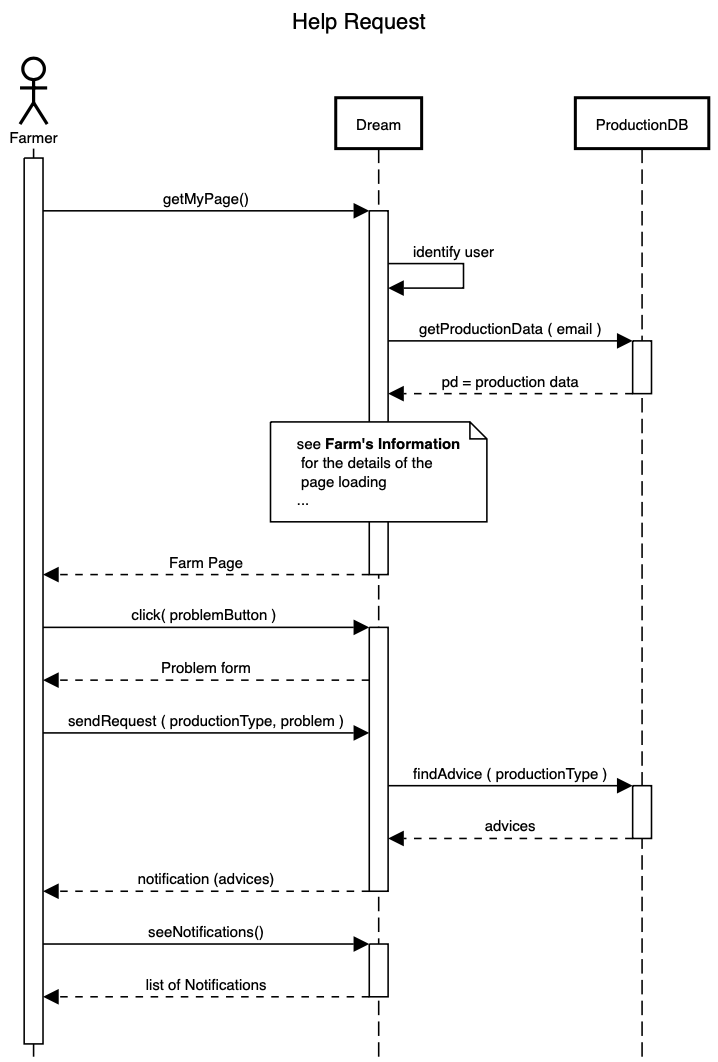
\includegraphics[width=0.7\textwidth]{sequence/HelpRequest.png}
        \caption{\emph{Farmer ask for help} sequence diagram}
        \label{fig:sequence6}
        \end{center}
    \end{figure}

    \item Submit an advice
    \begin{longtable}{p{0.26\linewidth}p{0.75\linewidth}}
        \toprule
        \textbf{Name} & \textbf{Farmer submits an advice} \\
        \midrule
        \textbf{Actors} & Farmer \\
        \midrule
        \textbf{Entry conditions} & The farmer has logged in\\
        \midrule
        \textbf{Flow of events} & 
        \begin{enumerate}
            \item The farmer has to submit an advice 
            \item The farmer clicks on his own page button
            \item The farmer clicks on Advice button
            \item The farmer chooses the type of production on which he wants to give advices
            \item The farmer fills the form writing his advice
            \item The farmer clicks submit button and sends the message
            \item The system saves the advice in the database
            \item The system notifies the farmer that the operation went succesfully 
        \end{enumerate} \\
        \midrule
        \textbf{Exit conditions} & The farmer submit an advice\\
        \midrule
        \textbf{Exceptions} & 
        \begin{itemize}
            \item If the farmer is not a "good" one the system doesn't save the advice and nottifies the farmer with an error message
        \end{itemize}\\
        \bottomrule
        \caption{\emph{Farmer send advice} use case description}
    \end{longtable}
    \begin{figure}[H]
        \begin{center}
        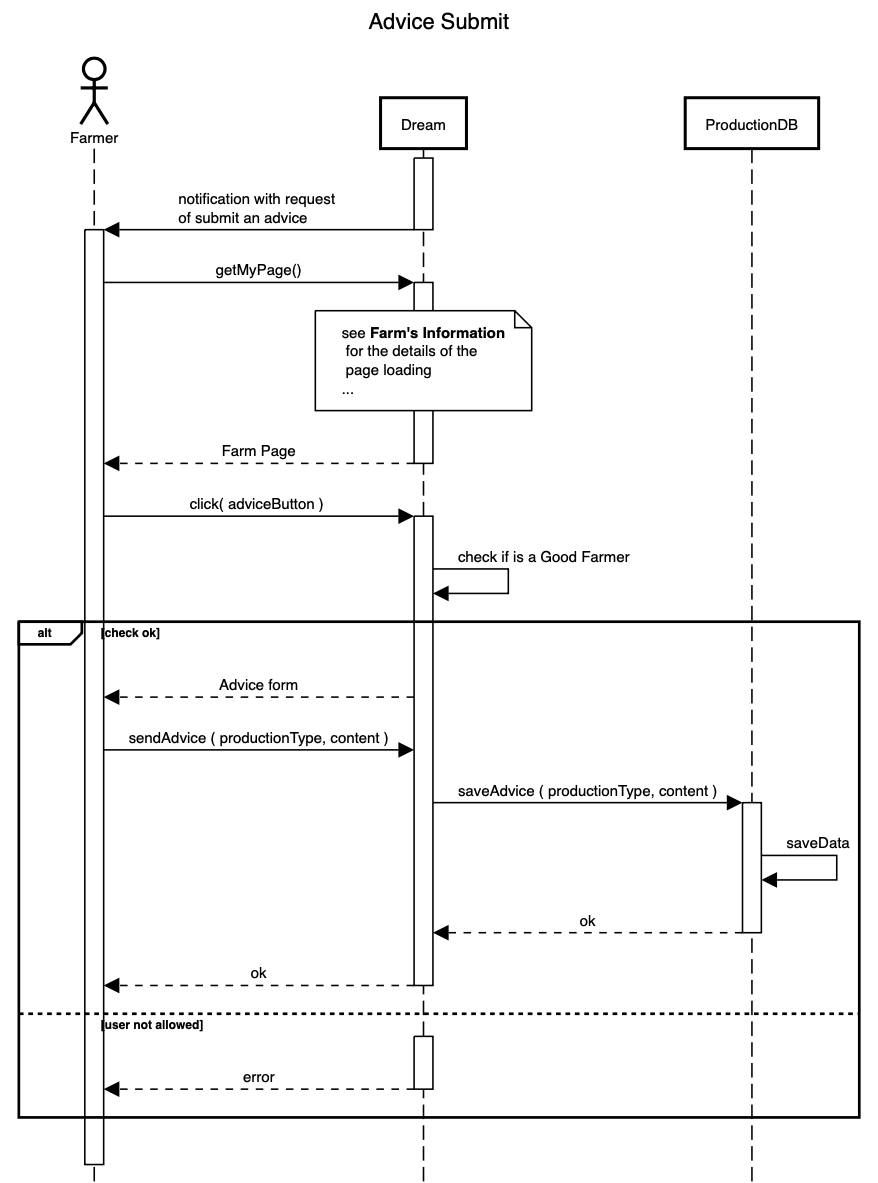
\includegraphics[width=0.7\textwidth]{sequence/AdviceSubmit.png}
        \caption{\emph{Farmer send advice} sequence diagram}
        \label{fig:sequence7}
        \end{center}
    \end{figure}

    \item Visualize notifications
    \begin{longtable}{p{0.26\linewidth}p{0.75\linewidth}}
        \toprule
        \textbf{Name} & \textbf{Farmer visualizes his notifications} \\
        \midrule
        \textbf{Actors} & Farmer \\
        \midrule
        \textbf{Entry conditions} & The farmer has logged in\\
        \midrule
        \textbf{Flow of events} & 
        \begin{enumerate}
            \item The farmer wants to read his notifications
            \item The farmer clicks on his own page button
            \item The farmer clicks on Notification button
            \item The system returns a list of messages
            \item The farmer selects one message between the ones in the list
            \item The system returns the body of the message
        \end{enumerate} \\
        \midrule
        \textbf{Exit conditions} & The farmer visualizes his notifications\\
        \midrule
        \textbf{Exceptions} & 
        \begin{itemize}
            \item 
        \end{itemize}\\
        \bottomrule
        \caption{\emph{Farmer visualize notifications} use case description}
    \end{longtable}
    \begin{figure}[H]
        \begin{center}
        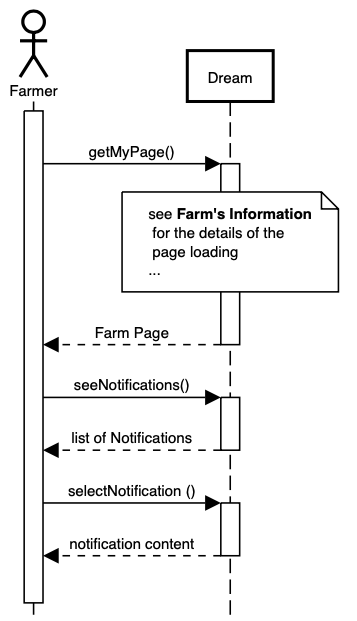
\includegraphics[width=0.7\textwidth]{sequence/SeeNotifications.png}
        \caption{\emph{Farmer visualize notifications} sequence diagram}
        \label{fig:sequence8}
        \end{center}
    \end{figure}

    \item Policy Maker login
    \begin{longtable}{p{0.26\linewidth}p{0.75\linewidth}}
        \toprule
        \textbf{Name} & \textbf{Farmer visualizes their own data} \\
        \midrule
        \textbf{Actors} & Policy Maker \\
        \midrule
        \textbf{Entry conditions} & The web application has started\\
        \midrule
        \textbf{Flow of events} & 
        \begin{enumerate}
            \item The Policy Maker wants to log in 
            \item The Policy Maker inserts code and password
            \item The Policy Maker clicks the submit button
            \item The system checks if the credentials are correct
            \item The system notifies the Policy Maker about the correct login
        \end{enumerate} \\
        \midrule
        \textbf{Exit conditions} & The Policy Maker has logged in\\
        \midrule
        \textbf{Exceptions} & 
        \begin{itemize}
            \item If the system does not recognize the code it will send an alert  to the Policy Maker saying that the code inserted is wrong
            \item If the password is not correct the system will notify the Policy Maker 
        \end{itemize}\\
        \bottomrule
        \caption{\emph{Policy Maker login} use case description}
    \end{longtable}
    \begin{figure}[H]
        \begin{center}
        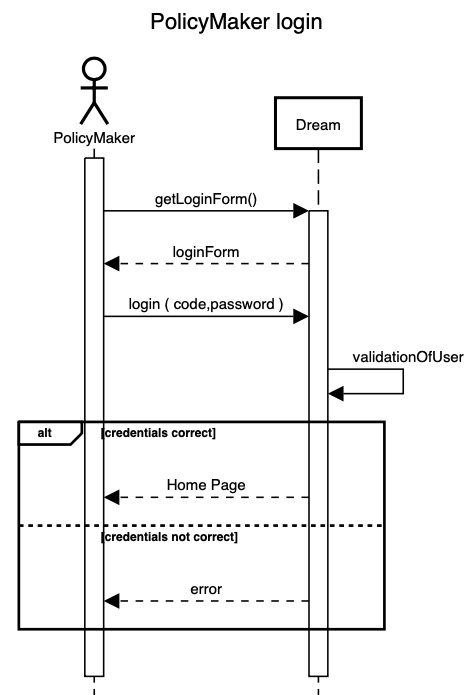
\includegraphics[width=0.7\textwidth]{sequence/PolicyMakerLogin.png}
        \caption{\emph{Policy Maker login} sequence diagram}
        \label{fig:sequence9}
        \end{center}
    \end{figure}

    \item Find a farm's page
    \begin{longtable}{p{0.26\linewidth}p{0.75\linewidth}}
        \toprule
        \textbf{Name} & \textbf{Policy Maker visualizes a farm’s page} \\
        \midrule
        \textbf{Actors} & Policy Maker \\
        \midrule
        \textbf{Entry conditions} & The Policy Maker has logged in\\
        \midrule
        \textbf{Flow of events} & 
        \begin{enumerate}
            \item The Policy Maker wants to visualize a farm's page
            \item The Policy Maker types the name of the farm on the search form
            \item The Policy Maker clicks search button
            \item The system redirects the Policy Maker to the farm's page
        \end{enumerate} \\
        \midrule
        \textbf{Exit conditions} & The Policy Maker visualizes the farm's page\\
        \midrule
        \textbf{Exceptions} & 
        \begin{itemize}
            \item If no name is inserted in the search form the system notifies the Policy Maker about the missing data
            \item If the name inserted is not present in the system's database, the system sends an error message
        \end{itemize}\\
        \bottomrule
        \caption{\emph{Farm’s page visualization} use case description}
    \end{longtable}
    \begin{figure}[H]
        \begin{center}
        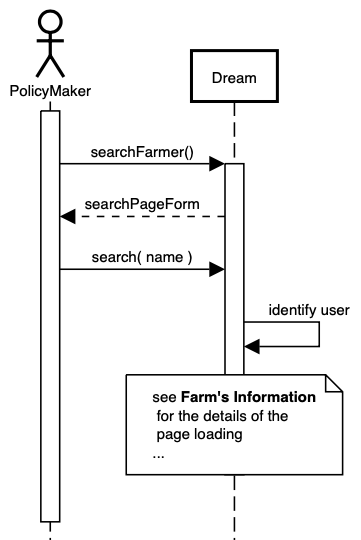
\includegraphics[width=0.7\textwidth]{sequence/PolicyMakerseachFarm.png}
        \caption{\emph{Farm’s page visualization} sequence diagram}
        \label{fig:sequence10}
        \end{center}
    \end{figure}

    \item Find a farmer on the Map
    \begin{longtable}{p{0.26\linewidth}p{0.75\linewidth}}
        \toprule
        \textbf{Name} & \textbf{Policy Maker visualizes a farm’s page} \\
        \midrule
        \textbf{Actors} & Policy Maker \\
        \midrule
        \textbf{Entry conditions} & The Policy Maker has logged in\\
        \midrule
        \textbf{Flow of events} & 
        \begin{enumerate}
            \item The Policy Maker wants to visualize the map
            \item The Policy Maker clicks on map button
            \item The system redirects the Policy Maker to the map page
            \item The Policy Maker visualizes the map and selects a farm
            \item The system retrieves the information about the farm (also the last evaluation) and shows them to the Policy Maker
            \item The Policy Maker visualizes the data about the selected farm
        \end{enumerate} \\
        \midrule
        \textbf{Exit conditions} & The Policy Maker visualizes his own data\\
        \midrule
        \textbf{Exceptions} & 
        \begin{itemize}
            \item 
        \end{itemize}\\
        \bottomrule
        \caption{\emph{Farm visualization on map} use case description}
    \end{longtable}
    \begin{figure}[H]
        \begin{center}
        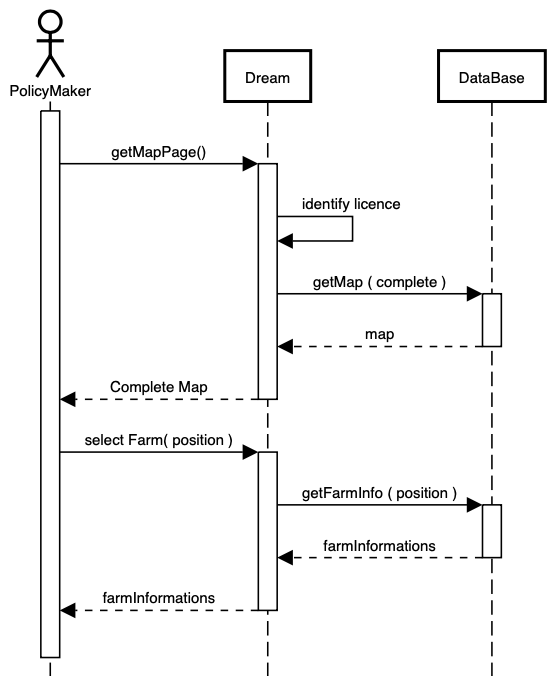
\includegraphics[width=0.7\textwidth]{sequence/searchOnMap.png}
        \caption{\emph{Farm visualization on map} sequence diagram}
        \label{fig:sequence11}
        \end{center}
    \end{figure}

    \item Update the Map
    \begin{longtable}{p{0.26\linewidth}p{0.75\linewidth}}
        \toprule
        \textbf{Name} & \textbf{Policy Maker update the map} \\
        \midrule
        \textbf{Actors} & Policy Maker \\
        \midrule
        \textbf{Entry conditions} & The Policy Maker has logged in\\
        \midrule
        \textbf{Flow of events} & 
        \begin{enumerate}
            \item The Policy Maker wants to report an evaluation
            \item The Policy Maker clicks on the map button
            \item The system redirects the Policy Maker to the map page
            \item The Policy Maker visualizes the map and selects a farm
            \item The system retrieves the information about the farm (also the last evaluation) and shows them to the Policy Maker
            \item The Policy Maker clicks update button
            \item The Policy Maker select the evaluation
                \begin{itemize}
                    \item The Policy Maker selects "good", decides an amount of money for the award and writes the body of the message
                    \item The Policy Maker selects "bad" and writes the body of the message
                \end{itemize}
            \item The Policy Maker clicks submit button and sends the message
            \item The system saves the evaluation on the map
            \item The system sends the message to the Farm's owner
            \item The system notifies the Policy Maker that the operation went succesfully 
        \end{enumerate} \\
        \midrule
        \textbf{Exit conditions} & The Policy Maker visualizes the map updated\\
        \midrule
        \textbf{Exceptions} & 
        \begin{itemize}
            \item 
        \end{itemize}\\
        \bottomrule
        \caption{\emph{Map updating} use case description}
    \end{longtable}
    \begin{figure}[H]
        \begin{center}
        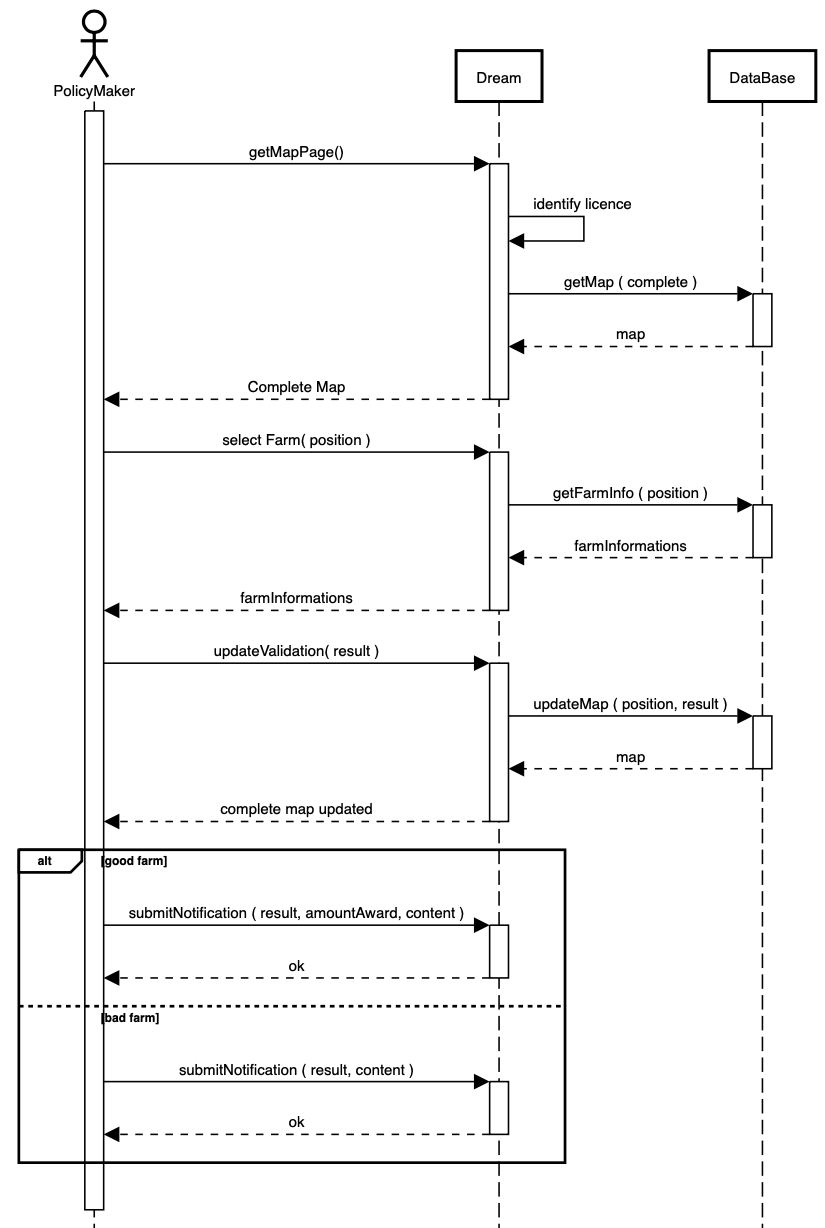
\includegraphics[width=0.7\textwidth]{sequence/updateMap.png}
        \caption{\emph{Map updating} sequence diagram}
        \label{fig:sequence12}
        \end{center}
    \end{figure}

    \item Reply to a request of help
    \begin{longtable}{p{0.26\linewidth}p{0.75\linewidth}}
        \toprule
        \textbf{Name} & \textbf{Policy Maker send anvice} \\
        \midrule
        \textbf{Actors} & Policy Maker \\
        \midrule
        \textbf{Entry conditions} & The Policy Maker has logged in\\
        \midrule
        \textbf{Flow of events} & 
        \begin{enumerate}
            \item The Policy Maker wants to send specific advices to a farmer
            \item The Policy Maker wants to see the informationabout a farm
            \item The Policy Maker types the name of the farm on search form
            \item The Policy Maker clicks search button 
            \item The Policy Maker wants to see the advices stored in the database on the type of production the farmers asked for help on
            \item The Policy Maker analyzes the data 
            \item The Policy Maker selects the farmer (name) and the type of production and writes the solution he found
            \item The Policy Maker clicks send button
            \item The system sends the message to the farmer
            \item The system notifies the Policy Maker that the operation was succesful
        \end{enumerate} \\
        \midrule
        \textbf{Exit conditions} & The Policy Maker send solutions\\
        \midrule
        \textbf{Exceptions} & 
        \begin{itemize}
            \item 
        \end{itemize}\\
        \bottomrule
        \caption{\emph{Problem resolution} use case description}
    \end{longtable}
    \begin{figure}[H]
        \begin{center}
        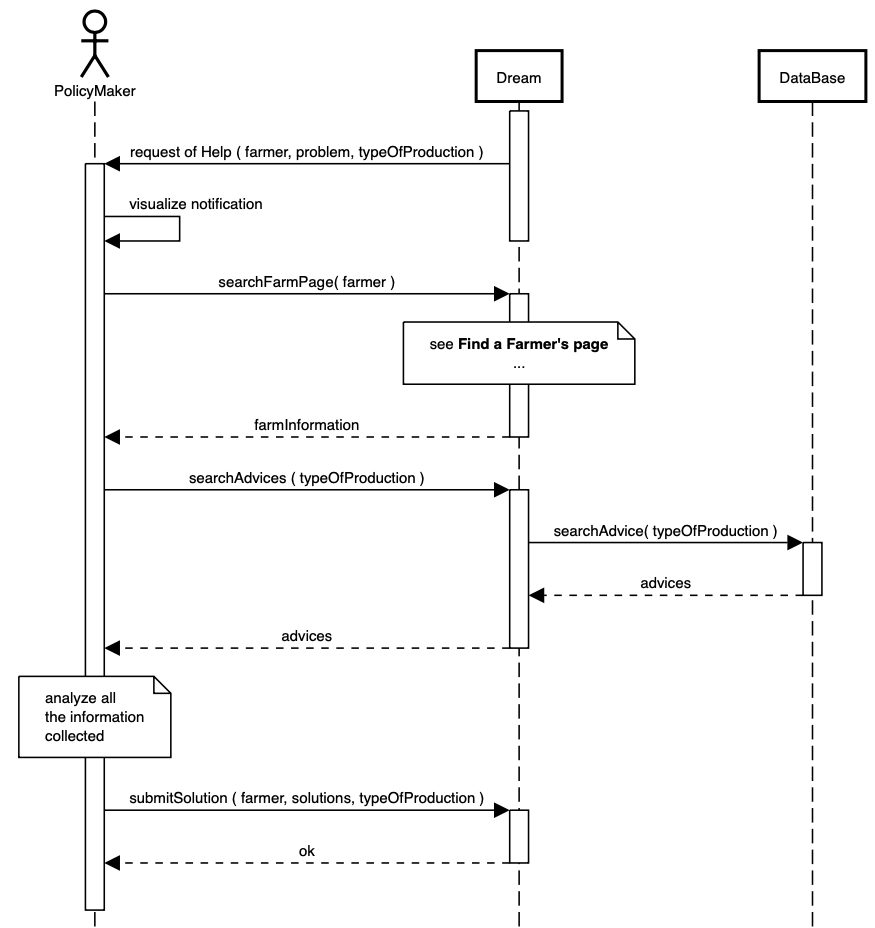
\includegraphics[width=0.7\textwidth]{sequence/replyHelp.png}
        \caption{\emph{Problem resolution} sequence diagram}
        \label{fig:sequence13}
        \end{center}
    \end{figure}
\end{enumerate}

%-----------------------------------------------------------------------------------%
\subsubsection{Scenarios}
\begin{enumerate}
    \item \textbf{Scenario 1}\\
    Dayanita is a young woman that lives in Singaram, a small town in the state of Telengana in India. 
    She lives with her parents in their family's farm. \\
    Their farm was mostly used to cultivate rice, so they are not really expert in other types of crop. She decides to try to expand their business, starting to grow 
    soyabean but her parents do not really know how to help her with it. \\
    Dayanita discovers, thanks to an ad she found online, a new web application that has been recently released. \\
    Therefore she decides to sign up and write a message on the forum hoping that some other farmer can share with her some advices.\\
    Ajar, the owner of Ajar's farm, answered her message saying to be careful and check the weather condition before planting the seeds and some suggestions 
    about the appropriate depth for planting them. 
    Dayainita some days later checks the forum again and reads Ajar's message. 
    The following days she checks the weather forecast that is present on her personalized farm page and actually 
    finds the right period to start planting soyabean.



    \item \textbf{Scenario 2}\\
    Nanuk is a Telengana’s policy maker. Dream IT providers distributed to each policy maker 
    reported by Telengana's government a secret code. Through this code 
    and password Nanuk is able to log in to Dream web application. 
    Before the 10th of the month all the policy makers are suppose to update the past evaluation 
    of the farms already present in 
    the system and add the farms that are added in the system in the past month.
    Using Dream the Nanuk searches on the map the farms that already been evaluated last month. 
    He finds out that Shaila's Farm did 
    not perform that well last time it was evaluated.
    Thus he decides to see if her performance is improved in the last month, he check the quantity 
    of wheat producted and 
    saw it increased dramatically from the month before.
    Therefore he decides to classify the farm as GOOD with a small incentive so that the owner 
    of the farm is stimulated to keep on doing good.
    
    
    \item \textbf{Scenario 3}\\
    Yamir is struggling with his Sesame crop. He tried everything, but still can not grow a quantity 
    that could increase his profit. \\
    His friend Ishaan only grows corn so he said he could not help him with it. However he suggested him to try to sign up to Dream 
    saying that there are a lot of ways he could get support from there. \\
    After he signed up he tried to write a message on the forum but nobody answered his text. 
    So he sent a request of help to the policy makers and finally discovered that he need to give more water to his plants.

    \item \textbf{Scenario 4}\\
    A policy maker working for Telengana's government is working with Dream application. The policy maker logs in with his code and password 
    to check his notification. The first notification he notices is a new request of help from Ajar's farm. He then looks at Ajar's farm page to look up all the information.
    Ajar is looking for suggestions on his wheat crop. The policy maker at this point send the solution of Ajar's problem, 
    filtering for type of production: wheat. 
    He reads all the advices written by other farmers and chooses the one written by Denali: wheat should be 
    planted in autumn or spring not in the other seasons. The policy maker writes then the solution and sends it to the farmer Ajar.

    
    
\end{enumerate}


%-----------------------------------------------------------------------------------%
\subsubsection{Requirements}
\textbf{R1} The system must allow farmers to register\\
\textbf{R2} The system must allow farmers to log in\\
\textbf{R3} The system must save the farmers registration data\\
\textbf{R4} The system must guarantee that each email address is unique\\
\textbf{R5} The system must verify that the email address is valid (the type!)\\
\textbf{R6} The system must save the farmers information about their production submitted\\
\textbf{R7} The system must allow farmers to insert the type of production \\
\textbf{R8} The system must allow farmers to insert the amount of production type\\
\textbf{R9} The system must allow farmers to specify a problem they faced to the Policy Makers\\
\textbf{R10} The system must allow farmers to select the type of production on which they had troubles\\
\textbf{R11} The system must save the advice submitted by the farmers\\
\textbf{R12} The system must allow farmers to select the type of product in their suggestion\\
\textbf{R13} The system must be able to show to the farmers advices send by the Policy Makers (as a notification)\\
\textbf{R14} The system must be able to show the meteorological data of the Farm’s position\\
\textbf{R15} The system must be able to show the farm’s sensor data \\
\textbf{R16} The system must allow farmers to send messages on the forum\\
\textbf{R17} The system must register date and time of a message in the forum\\
\textbf{R18} The system must be able to show all the messages on the forum\\
\textbf{R19} The system must be able to show the map of the zone\\
\textbf{R20} The system must be able to show the farms position on the map\\
\textbf{R21} the system must be able to show on the map if a farm is performing well or not \\
\textbf{R22} The system must allow farmers to visualise notification send by Policy Makers\\
\textbf{R23} The system must allow farmers to see all information about his own farm\\
\textbf{R24} The system must be able to show the types of production cultivated in a farm\\
\textbf{R25} The system must be able to show the quantity of product has been cultivated for each type in a farm\\
\textbf{R26} The system does not allow Policy Makers to register\\
\textbf{R27} The system must allow Policy Makers to log in\\
\textbf{R28} The system must verify that the code is valid\\
\textbf{R29} The system must allow Policy Makers to search a farm by name (OK?)\\
\textbf{R30} The system must allow Policy Makers to see all farms’ pages\\
\textbf{R31} The system must not allow Policy Makers to modify any farm’s page\\
\textbf{R32} The system must allow Policy Makers to update the performance of a farmer\\
\textbf{R33} The system must allow Policy Makers to send notification to the farmers\\
\textbf{R34} The system must allow Policy Makers to receive request of help by the farmers\\
%-----------------------------------------------------------------------------------%
\newpage

\subsubsection{Goals}

\begin{table}[ht]

\begin{center}

\begin{tabular}{|p{2cm}|p{4cm}|p{4cm}|}
    
    \toprule
   Goals & Domain Assumpitons & Requirements \\
   \midrule
    G1 & DA1, DA2, DA3, DA4, DA5, DA6, DA7, DA8, DA9, DA13, DA16, DA18 & R14, R15, R26, R27, R28, R29, R30, R31, R32 \\ 
    \midrule
    G2 & DA1, DA4, DA6, DA10, DA15, DA17 & R1, R2, R3, R4, R5, R16, R17, R18 \\
    \midrule
    G3 & DA1, DA2, DA6, DA9, DA12, DA14, DA15, DA17 & R1, R2, R3, R4, R5, R6, R7, R8, R11, R12 \\
    \midrule
    G4 & DA1, DA6, DA9, DA11, DA15, DA17 & R1, R2, R3, R4, R5, R9, R10, R13, R22, R33, R34 \\
    \midrule
    G5 & DA1, DA3, DA4, DA5, DA6, DA7, DA8, DA9, DA10, DA13, DA15, DA17 & R1, R2, R3, R4, R5, R14, R15, R22, R23, R24, R25 \\
    \midrule
    G6A & DA1, DA5, DA6, DA8, DA9, DA15, DA16, DA17 & R1, R2, R3, R4, R5, R19, R20, R26, R27, R28 \\
    \midrule
    G6B & DA1, DA2, DA5, DA6, DA8, DA9, DA13, DA15, DA16, DA17 & R19, R20, R21, R24, R25, R26, R27, R28, R32, R33 \\
    \midrule
    G6C & DA1, DA2, DA5, DA6, DA8, DA9, DA15, DA16, DA17 & R1, R2, R3, R4, R5, R19, R20, R24 \\
    \bottomrule
\end{tabular}
\end{center}
\caption{Mapping of goals, domain assumptions and requirements}
\end{table}



\begin{itemize}   
    \item \textbf{G1} Allow Policy Makers to retrieve information about a farm and to evaluate their performance
        \begin{itemize}
            \renewcommand\labelitemi{--}
            \item \textbf{R14} The system must be able to show the meteorological data of the Farm’s position
            \item \textbf{R15} The system must be able to show the farm’s sensor data
            \item \textbf{R26} The system does not allow Policy Makers to register
            \item \textbf{R27} The system must allow Policy Makers to log in
            \item \textbf{R28} The system must verify that the code is valid
            \item \textbf{R29} The system must allow Policy Makers to search a farm by name
            \item \textbf{R30} The system must allow Policy Makers to see all farms’ pages
            \item \textbf{R31} The system must not allow Policy Makers to modify any farm’s page
            \item \textbf{R32} The system must allow Policy Makers to update the performance of a farmer
            \item \textbf{DA1} In order to access the system users need to have Internet connection
            \item \textbf{DA2} Farmers always insert correct data on their production activity
            \item \textbf{DA3} Data from sensors is always correct
            \item \textbf{DA4} Date and Time on the system are always correct
            \item \textbf{DA5} The position of the Farm is always correct
            \item \textbf{DA6} Internet connection works always without errors
            \item \textbf{DA7} Meteorological data is accurate
            \item \textbf{DA8} Every farm has a different position
            \item \textbf{DA9} Each farm belongs to exacly one farmer
            \item \textbf{DA13} Performances of farmers are always identified correctly
            \item \textbf{DA16} Policy Makers have a given code and password to access the system
            \item \textbf{DA18} The special incentive that the farmers received for their good work, is used on stuff related to their production
        \end{itemize}
    
    \item \textbf{G2} Allow farmer to comunicate with each other
        \begin{itemize}
            \renewcommand\labelitemi{--}
            \item \textbf{R1} The system must allow farmers to register
            \item \textbf{R2} The system must allow farmers to log in
            \item \textbf{R3} The system must save the farmers registration data
            \item \textbf{R4} The system must guarantee that each email address is unique
            \item \textbf{R5} The system must verify that the email address is valid
            \item \textbf{R16} The system must allow farmers to send messages on the forum
            \item \textbf{R17} The system must register date and time of a message in the forum
            \item \textbf{R18} The system must be able to show all messages on the forum
            \item \textbf{DA1} In order to access the system users need to have Internet connection
            \item \textbf{DA4} Date and Time on the system are always correct
            \item \textbf{DA6} Internet connection works always without errors
            \item \textbf{DA10} Discussion on the forum are related only to the farm activity
            \item \textbf{DA15} The email and farm's name must be unique
            \item \textbf{DA17} All farmers that sign up own a real farm in Telengana
        \end{itemize}    
    
    \item \textbf{G3} Allow farmer to insert data and advices on his production
        \begin{itemize}
        \renewcommand\labelitemi{--}
        \item \textbf{R1} The system must allow farmers to register
        \item \textbf{R2} The system must allow farmers to log in
        \item \textbf{R3} The system must save the farmers registration data
        \item \textbf{R4} The system must guarantee that each email address is unique
        \item \textbf{R5} The system must verify that the email address is valid
        \item \textbf{R6} The system must save the farmers information about their production submitted
        \item \textbf{R7} The system must allow farmers to insert the type of production
        \item \textbf{R8} The system must allow farmers to insert the amount of production type
        \item \textbf{R11} The system must save the advice submitted by the farmers
        \item \textbf{R12} The system must allow farmers to select the type of product in their suggestion
        \item \textbf{DA1} In order to access the system users need to have Internet connection
        \item \textbf{DA2} Farmers always insert correct data on their production activity
        \item \textbf{DA6} Internet connection works always without errors
        \item \textbf{DA9} Each farm belongs to exacly one farmer
        \item \textbf{DA12} Advice on a product must be given by a farmer that produces the same type
        \item \textbf{DA14} Farmers can insert data more than once a day
        \item \textbf{DA15} The email and farm's name must be unique
        \item \textbf{DA17} All farmers that sign up own a real farm in Telengana
        \end{itemize} 
    
    \item \textbf{G4} Allow farmer to send request of help to Policy Makers
        \begin{itemize}
        \renewcommand\labelitemi{--}
        \item \textbf{R1} The system must allow farmers to register
        \item \textbf{R2} The system must allow farmers to log in
        \item \textbf{R3} The system must save the farmers registration data
        \item \textbf{R4} The system must guarantee that each email address is unique
        \item \textbf{R5} The system must verify that the email address is valid
        \item \textbf{R9} The system must allow farmers to specify a problem they faced to the Policy Makers
        \item \textbf{R10} The system must allow farmers to select the type of production on which they had troubles
        \item \textbf{R13} The system must be able to show to the farmers advices send by the Policy Makers
        \item \textbf{R22} The system must allow farmers to visualise notification send by Policy Makers
        \item \textbf{R33} The system must allow Policy Makers to send notification to the farmers
        \item \textbf{R34} The system must allow Policy Makers to receive request of help by the farmers
        \item \textbf{DA1} In order to access the system users need to have Internet connection
        \item \textbf{DA6} Internet connection works always without errors
        \item \textbf{DA9} Each farm belongs to exacly one farmer
        \item \textbf{DA11} Formal request of help must be related to a farmer's own production
        \item \textbf{DA15} The email and farm's name must be unique
        \item \textbf{DA17} All farmers that sign up own a real farm in Telengana
        \end{itemize} 
    
    \item \textbf{G5} Allow farmers to retrieve information relevant for their activity
        \begin{itemize}
        \renewcommand\labelitemi{--}
        \item \textbf{R1} The system must allow farmers to register
        \item \textbf{R2} The system must allow farmers to log in
        \item \textbf{R3} The system must save the farmers registration data
        \item \textbf{R4} The system must guarantee that each email address is unique
        \item \textbf{R5} The system must verify that the email address is valid
        \item \textbf{R14} The system must be able to show the meteorological data of the Farm’s position
        \item \textbf{R15} The system must be able to show the farm’s sensor data
        \item \textbf{R22} The system must allow farmers to visualise notification send by Policy Makers
        \item \textbf{R23} The system must allow farmers to see all information about his own farm
        \item \textbf{R24} The system must be able to show the types of production cultivated in a farm
        \item \textbf{R25} The system must be able to show the quantity of product has been cultivated for each type in a farm
        \item \textbf{DA1} In order to access the system users need to have Internet connection
        \item \textbf{DA3} Data from sensors is always correct
        \item \textbf{DA4} Date and Time on the system are always correct
        \item \textbf{DA5} The position of the Farm is always correct
        \item \textbf{DA6} Internet connection works always without errors
        \item \textbf{DA7} Meteorological data is accurate
        \item \textbf{DA8} Every farm has a different position
        \item \textbf{DA9} Each farm belongs to exacly one farmer
        \item \textbf{DA10} Discussion on the forum are related only to the farm activity
        \item \textbf{DA13} Performances of farmers are always identified correctly
        \item \textbf{DA15} The email and farm's name must be unique
        \item \textbf{DA17} All farmers that sign up own a real farm in Telengana
        \end{itemize} 
        
    \item \textbf{G6} Policy Makers and farmers should be able to consult the map of the zone ( and the informations stored in it ) with different levels of visibility
        \begin{enumerate}
            \item \textbf{G6A} Policy Makers and farmers should be able to see the position of the farms on the map
            \begin{itemize}
                \renewcommand\labelitemi{--}
                \item\textbf{R1} The system must allow farmers to register
                \item\textbf{R2} The system must allow farmers to log in
                \item\textbf{R3} The system must save the farmers registration data
                \item\textbf{R4} The system must guarantee that each email address is unique
                \item\textbf{R5} The system must verify that the email address is valid
                \item\textbf{R19} The system must be able to show the map of the zone
                \item\textbf{R20} The system must be able to show the farms position on the map
                \item\textbf{R26} The system does not allow Policy Makers to register
                \item\textbf{R27} The system must allow Policy Makers to log in
                \item\textbf{R28} The system must verify that the code is valid
                \item\textbf{DA1} In order to access the system users need to have Internet connection
                \item\textbf{DA5} The position of the Farm is always correct
                \item\textbf{DA6} Internet connection works always without errors
                \item \textbf{DA8} Every farm has a different position
                \item \textbf{DA9} Each farm belongs to exacly one farmer
                \item \textbf{DA15} The email and farm's name must be unique
                \item \textbf{DA16} Policy Makers have a given code and password to access the system
                \item \textbf{DA17} All farmers that sign up own a real farm in Telengana
            \end{itemize}
            \item\textbf{G6B} Policy Makers should be able to see both the information about the production and the evaluation of each farm
            \begin{itemize}
                \renewcommand\labelitemi{--}
                \item \textbf{R19} The system must be able to show the map of the zone
                \item \textbf{R20} The system must be able to show the farms position on the map
                \item \textbf{R21} The system must be able to show on the map if a farm is performing well or not
                \item \textbf{R24} The system must be able to show the types of production cultivated in a farm
                \item \textbf{R25} The system must be able to show the quantity of product has been cultivated for each type in a farm
                \item \textbf{R26} The system does not allow Policy Makers to register
                \item \textbf{R27} The system must allow Policy Makers to log in
                \item \textbf{R28} The system must verify that the code is valid
                \item \textbf{R32} The system must allow Policy Makers to update the performance of a farmer
                \item \textbf{R33} The system must allow Policy Makers to send notification to the farmers
                \item \textbf{DA1} In order to access the system users need to have Internet connection
                \item \textbf{DA2} Farmers always insert correct data on their production activity
                \item \textbf{DA5} The position of the Farm is always correct
                \item \textbf{DA6} Internet connection works always without errors
                \item \textbf{DA8} Every farm has a different position
                \item \textbf{DA9} Each farm belongs to exacly one farmer
                \item \textbf{DA13} Performances of farmers are always identified correctly
                \item \textbf{DA15} The email and farm's name must be unique
                \item \textbf{DA16} Policy Makers have a given code and password to access the system
                \item \textbf{DA17} All farmers that sign up own a real farm in Telengana
            \end{itemize}    
            \item \textbf{G6C} Farmers should be able to see only the type of production of a farmer by the map
            \begin{itemize}
                \renewcommand\labelitemi{--}
                \item \textbf{R1} The system must allow farmers to register
                \item \textbf{R2} The system must allow farmers to log in
                \item \textbf{R3} The system must save the farmers registration data
                \item \textbf{R4} The system must guarantee that each email address is unique
                \item \textbf{R5} The system must verify that the email address is valid
                \item \textbf{R19} The system must be able to show the map of the zone
                \item \textbf{R20} The system must be able to show the farms position on the map
                \item \textbf{R24} The system must be able to show the types of production cultivated in a farm
                \item \textbf{DA1} In order to access the system users need to have Internet connection
                \item \textbf{DA2} Farmers always insert correct data on their production activity
                \item \textbf{DA5} The position of the Farm is always correct
                \item \textbf{DA6} Internet connection works always without errors
                \item \textbf{DA8} Every farm has a different position
                \item \textbf{DA9} Each farm belongs to exacly one farmer
                \item \textbf{DA15} The email and farm's name must be unique
                \item \textbf{DA16} Policy Makers have a given code and password to access the system
                \item \textbf{DA17} All farmers that sign up own a real farm in Telengana
                
            \end{itemize}
        \end{enumerate}
    \end{itemize}



%-----------------------------------------------------------------------------------%
\subsubsection{Traceability Matrix}
%-----------------------------------------------------------------------------------%
\subsection{Performance Requirements}
The system serves its user with a web application. All the computations will take place on the server side, 
thus the app is meant to be lightweighted. Moreover the load in the night is expected to be really low.
There are no problems about reliability. The insertion of new data requires a quick response in order to store 
it in the system.

%-----------------------------------------------------------------------------------%
\subsection{Design Constraints}
\subsubsection{Standards Compliance}
The only standard that needs to be highlighted here is the interaction with the database. It is important that the information are stored 
in a standardized form. In such manner, it is easier to memorize and retrieve data.


\subsubsection{Any Other Constraints}
Interaction between Dream and users needs to consider also regulatory policies.
As a matter of fact the application asks and retrieves data of each farmer.
More information about security and privacy will be provided in the section~\ref{subsubsection:3.4.3}


%-----------------------------------------------------------------------------------%
\subsection{Software System Attributes}

\subsubsection{Reliability}
The system must prevent any failure in order to guarantee continuity. 
Simultaneous accesses are expected to work, especially in the afternoon when users are expectd to insrt and retrieve more information.

\subsubsection{Availability}
It is expected that the system has the lowest downtime possible. 
The system is available with a minimum time of 96\%, 
so that it about 14 days a year of downtime are allowed.


\subsubsection{Security}
\label{subsubsection:3.4.3}
Security of the data and of the communication user-system is a primary concern. Users credential are stored in a data base, so the system crypt the password data before store it. The system recognises the right type of user during the log in phase to ensure providing the correct level visibility of the data and the permission to update them or not. In this way farmer’s privacy is guaranteed. As a matter of fact a farmer can’t see another farmer’s page.


\subsubsection{Maintanability}
The web application requires ordinary maintenance for improvements and in order to fix potential bugs. 
It is going to be scheduled at local night time, when user traffic is the lowest.
Moreover the system must be designed in a way that allows future addition of features.

\subsubsection{Portability}
The system as a web application must run on different software system as Windows, Linux an macOS.
On the server side is crucial focusing on the interaction between APIs and the data base to insert, update or read data.



%-----------------------------------------------------------%
\newpage
\section{Formal Analysis using Alloy}


%-----------------------------------------------------------%
\section{Effort Spent}

\end{document}
